% 设置编码,编码为UTF-8编码,字号大小12pt
\documentclass[UTF8, 12pt]{ctexart}
\usepackage{graphicx}
\usepackage{geometry}
\usepackage{titlesec}{\tiny}
\usepackage{amsmath}
\usepackage{authblk}
\usepackage{booktabs}
\usepackage{url}

% 定义超链接的颜色
\usepackage[colorlinks, linkcolor=blue, citecolor=blue]{hyperref}

% 标题左对齐
%\CTEXsetup[format={\Large\bfseries}]{section}

% 定义
\newtheorem{theorem}{Theorem}[section]
% 控制图片的位置,让图片紧紧的跟住文字,只需写\begin{figure}[H]
\usepackage{float}
% 使用文献引用
\usepackage{cite}
% 使用算法排版模块
\usepackage{algorithm}  
\usepackage{algorithmic}
\renewcommand{\algorithmicrequire}{\textbf{输入:}}  
\renewcommand{\algorithmicensure}{\textbf{输出:}} 
% 设置文本格式,文本间距等,具体参考如下:
% left=2cm, right=2cm, top=2.5cm,bottom=1.5cm
\geometry{a4paper, centering, scale=0.8}
\newtheorem{thm}{定义}
\renewcommand{\baselinestretch}{1.3}

% 定义编程语言
\usepackage{listings}
\usepackage{color}
\usepackage{fontspec}
\definecolor{dkgreen}{rgb}{0,0.6,0}
\definecolor{gray}{rgb}{0.5,0.5,0.5}
\definecolor{mauve}{rgb}{0.58,0,0.82}
\definecolor{light-gray}{gray}{0.95}

\lstset{frame=tb,
		language=Python,
		aboveskip=3mm,
		belowskip=1mm,
		showstringspaces=false,
		columns=flexible,
		basicstyle=\small\ttfamily,
		numbers=left,
		numberstyle=\small\color{gray},
		keywordstyle=\color{blue},
		commentstyle=\color{dkgreen},
		stringstyle=\color{mauve},
		breaklines=true,
		breakatwhitespace=true,
		tabsize=4,
		backgroundcolor=\color{light-gray}}

\begin{document}
	\title{\heiti \Huge{liu123的航空母舰队决赛说明文档}}
	\author{\kaishu 尹卓 \\ E-mails: \href{mailto:zhuoyin94@163.com}{zhuoyin94@163.com}}
	\date{\today}
	\maketitle

	% 增加目录
	\tableofcontents
	\newpage
	\section{团队成员简介}
		团队的主要队员来自研究机构、互联网公司和高校。表\ref{table_0}是团队成员的基本情况介绍。

		\begin{table}[H]
		\centering
		\small
		\caption{团队成员简介}
		\label{table_0}
		\renewcommand\arraystretch{0.9}
		\begin{tabular}{lllp{2.4cm}l}
			\toprule
			\textbf{姓名} & \textbf{单位} & \textbf{职位} & \textbf{研究方向} & \textbf{联系方式}\\
			\midrule
			尹卓\footnotemark[1] & 交控科技研究院 & 软件工程师 & 异常检测,时序数据挖掘 & \href{mailto:zhuoyin94@163.com}{zhuoyin94@163.com}\\
			刘震林 & 兰州大学 & 硕士研究生 & 数据挖掘 & - \\
			高璇颖 & 京东数科战略部 & 战略咨询师 & TMT行业战略规划与市场研究 & - \\
			刘义卿 & 北京工业大学 & 硕士研究生 & 图像处理,数据可视化 & - \\
			卢佳程 & 北京工业大学 & 硕士研究生 & 智能交通 & - \\
			\bottomrule
		\end{tabular}
		\end{table}
		\footnotetext[1]{队长,项目开源地址:\url{https://github.com/MichaelYin1994/tianchi-DCIC2020-trajectory-mining}}

		我们在初赛A阶段中排名\textbf{4/3275},初赛B阶段排名\textbf{37/3275};复赛算法A阶段排名\textbf{10/120},复赛算法B阶段排名\textbf{3/120};复赛可视化阶段排名\textbf{7/14}。我们所有工作在本地进行。设备配置为i9-97820X处理器,32G内存,系统环境为Ubuntu 18.04 LTS。本文档采用 \LaTeX 撰写。

	%%%%%%%%%%%%%%%%%%%%%%%%%%%%%%%%%%%%%%%%%%%%
	%%%%%%%%%%%%%%%%%%%%%%%%%%%%%%%%%%%%%%%%%%%%
	\section{背景分析与任务描述}
		\subsection{背景描述}
		我国海洋生产市场未来具有较大发展空间,而海上安全治理仍存在一定发展痛点与问题。活跃在我国专属经济海域的各类目标种类繁多、规模庞大,主要涵盖了渔船、商船、养殖渔排、网具等等。船舶避碰终端(AIS)、北斗定位终端等通信导航设备的应用,给海上交通和作业带来了极大便利, 但也产生了新的问题。设备信息不规范导致目标信息失真,进而使得商船误入养殖区、渔船碰撞商船等,造成巨大的人身和财产损失,为海上安全治理带来了极大挑战。

		以人工智能、大数据、区块链等新一代信息技术为支撑的智慧海洋,有望为这一问题提供解决方案。提升海上安全治理能力,首要任务是“看得清” ,即看得清“是什么、谁在用、做什么”,这也是本次比赛需要解决的核心问题。“是什么”指的是通过分析AIS设备位置数据,得出是哪一类目标在使用该设备;“谁在用”则是通过分析渔船北斗设备位置数据(船号清楚)和AIS设备位置数据(船号不清),得出是哪一艘船在使用该AIS设备; “做什么”就是通过分析渔船北斗设备位置数据,得出该船的生产作业行为,具体判断出是拖网作业、围网作业还是流刺网作业。

		DCIC 2020数字中国智慧海洋建设比赛分为两个阶段:第一阶段,要求选手基于位置数据对海上目标进行智能识别和作业行为分析,通过分析渔船北斗设备位置数据,得出该船的生产作业行为,具体判断出是拖网作业、围网作业还是流刺网作业。第二阶段,希望第一阶段TOP20选手通过数据可视分析,挖掘更多海洋通信导航设备的应用价值,构建渔船的用户画像,其中鼓励用可视化方式呈现。

		\subsection{任务简述}
		算法赛阶段,选手需要通过分析渔船北斗设备位置数据,建立机器学习模型来判断出该船的生产作业行为,到底是拖网作业(Class 0)、围网作业(Class 1)还是流刺网作业(Class 2),每条渔船轨迹包含经度、纬度、速度、方向、渔船id与时间戳这5维特征。其中,初赛提供11000条轨迹(7000线下训练,2000线上测试A,2000线上测试B);复赛提供了8166条轨迹用于线下训练,线上阿里云Dcoker环境包含4000条轨迹(2000测试A与2000测试B)。评分采用了预测的三种类别的F1值平均作为最终成绩:
		\begin{equation}
			score = \frac{F1_{class \; 0} + F1_{class \; 1} + F1_{class \; 2}}{3}
		\end{equation}
		其中初赛和复赛均为两阶段,第一阶段在数据集测试A上评估在训练集上训练的模型的分数,第二阶段更换线上测试集B,在测试集B上评估两次模型的分数,作为最终比赛成绩。

		复赛可视化阶段,主办方提供船舶的AIS数据(Automatic Identification System),该数据可视为不同数据源的渔船轨迹数据。主办方希望选手根据AIS数据充分挖掘海洋设备的更多应用价值,并进行可视化展现。

		\subsection{赛题难点}
		针对渔船轨迹数据挖掘问题,此次比赛存在以下几个难点:
		\begin{enumerate}
			\item \textbf{轨迹数据中存在各种各样的噪声:}首先不论是北斗轨迹还是AIS轨迹,均存在传感器采集精度导致的噪声;其次,船只的局部运动行为也会导致各种记录噪声的出现。
			\item \textbf{轨迹运动模式复杂:}相比较陆地GPS轨迹与监控场景的运动目标轨迹而言,海上运动目标不受几何结构约束,其运动模式较陆地目标更为复杂。
			\item \textbf{轨迹数据隐藏有较强的语义信息:}轨迹数据天生具有较强的语意信息,如何挖掘这样的语意信息强化模型的稳定性,并提升特征对渔船运动特性的刻画也是挖掘的难点。
		\end{enumerate}

		\subsection{文档结构}
		本文档主要介绍我们在算法阶段的数据分析与特征工程的相关工作。具体来说,第\ref{sec_1}章,介绍基于北斗轨迹的基础可视化信息研究;第\ref{sec_2}章介绍针对渔船作业类型分类的渔船基础统计特征的构建;第\ref{sec_3}章总结与展望未来的工作。

%%%%%%%%%%%%%%%%%%%%%%%%%%%%%%%%%%%%%%%%%%%%
%%%%%%%%%%%%%%%%%%%%%%%%%%%%%%%%%%%%%%%%%%%%
	\section{基础数据探索性分析}\label{sec_1}
	本阶段,我们着重探索复赛渔船北斗轨迹的基础统计信息,以获得基础的针对渔船轨迹的认识,便于后续的特征组织与可视化工作。

%%%%%%%%%%%%%%%%%%%%%%%%%%%%%%%%%%%%%%%%%%%%
	\subsection{针对渔船北斗轨迹的统计可视化研究}
	首先,我们从三类轨迹中随机挑选三条轨迹进行可视化。
	\begin{figure}[H]
		\centering
		\includegraphics[width=0.8\linewidth]{..//plots//traj_randomly_9_traj.png}
		\caption{随机挑选不同作业类型的3条北斗轨迹进行可视化}
		\label{sec_1_fig_0}
		\vspace{-0.2cm}
	\end{figure}
	图(\ref{sec_1_fig_0})是各个作业类别随机挑选的3条轨迹的可视化结果。其中,蓝色为Class 0,橙色为Class 1,绿色为Class 2。我们进一步将某条轨迹的经度与纬度信息按照时间序列的方式进行可视化,图(\ref{sec_1_fig_1})为某条轨迹的经纬度序列的可视化信息。
	\begin{figure}[H]
		\centering
		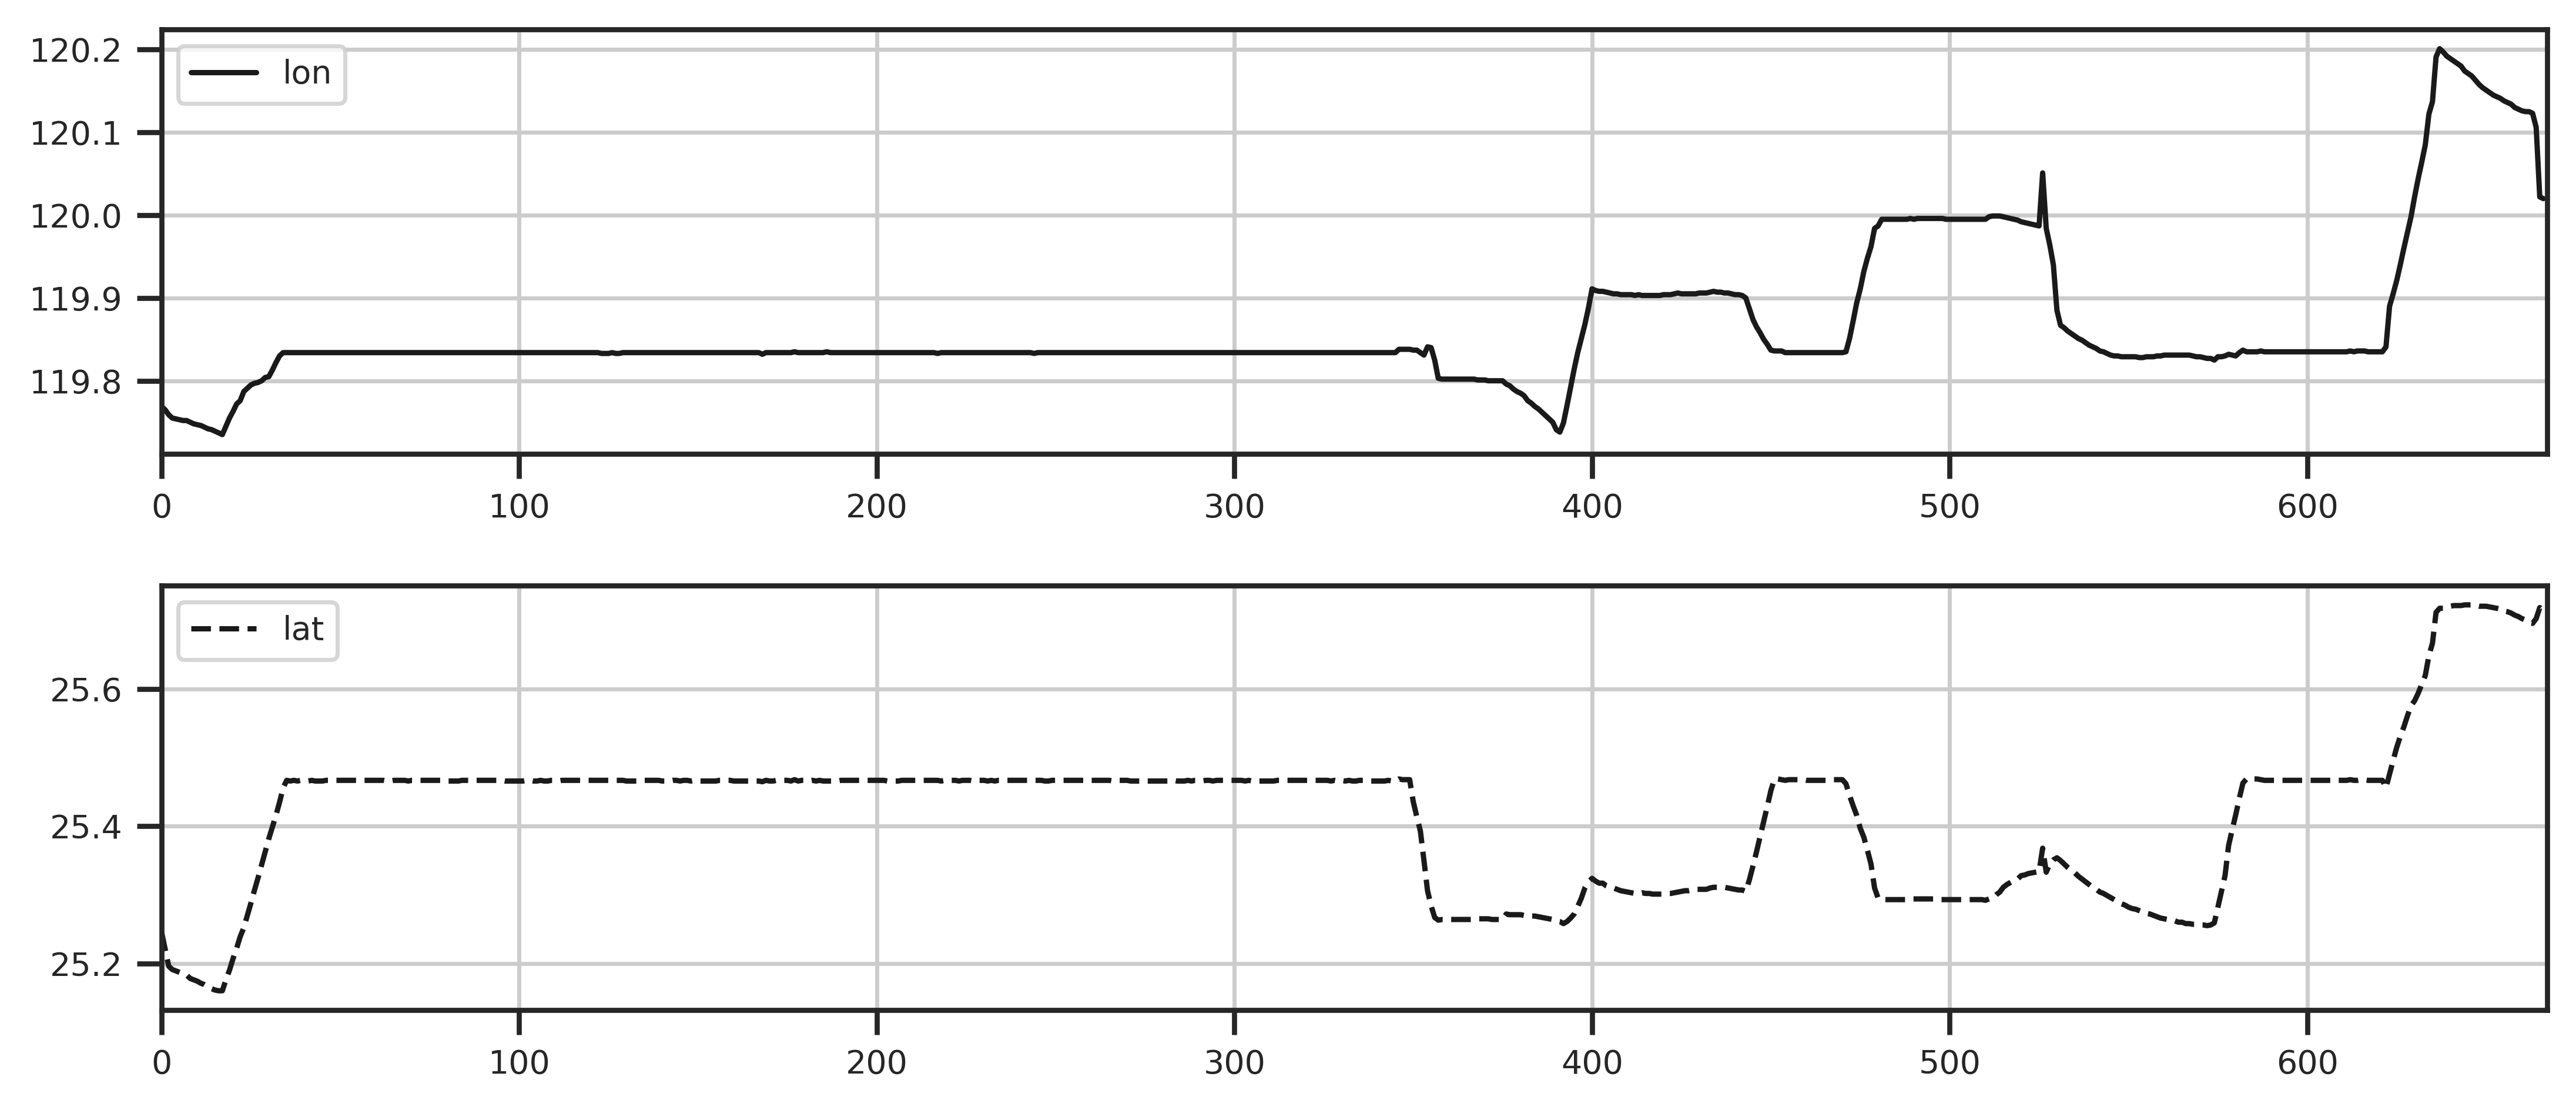
\includegraphics[width=0.7\linewidth]{..//plots//traj_lon_lat_sequence.png}
		\caption{渔船经度与纬度序列信息可视化}
		\label{sec_1_fig_1}
		\vspace{-0.2cm}
	\end{figure}
	由图(\ref{sec_1_fig_0})与图(\ref{sec_1_fig_1})可以得出以下结论:
	\begin{enumerate}
		\item \textbf{不同类别轨迹无直接可区分规律。}北斗轨迹形状复杂,通过图(\ref{sec_1_fig_0})对每条轨迹进行直接观察,没有明显的能够直接区分三种轨迹的规律存在。 
		\item \textbf{存在“异常”轨迹。}通过多次绘制图(\ref{sec_1_fig_0})可得,训练集内部存在大量直观感受异常的轨迹,例如某条轨迹包含600多个轨迹点,但只有几个不同的(Unique)的轨迹点。
		\item \textbf{轨迹存在POI点。}从图(\ref{sec_1_fig_1})单条轨迹的经纬度角度看,轨迹中存在POI点(Points of Interested),通过背景知识可知,在该场景下的POI点可能代表的是港口,也可能是海上刺网捕捞渔场的位置。
	\end{enumerate}

	\begin{figure}[H]
		\centering
		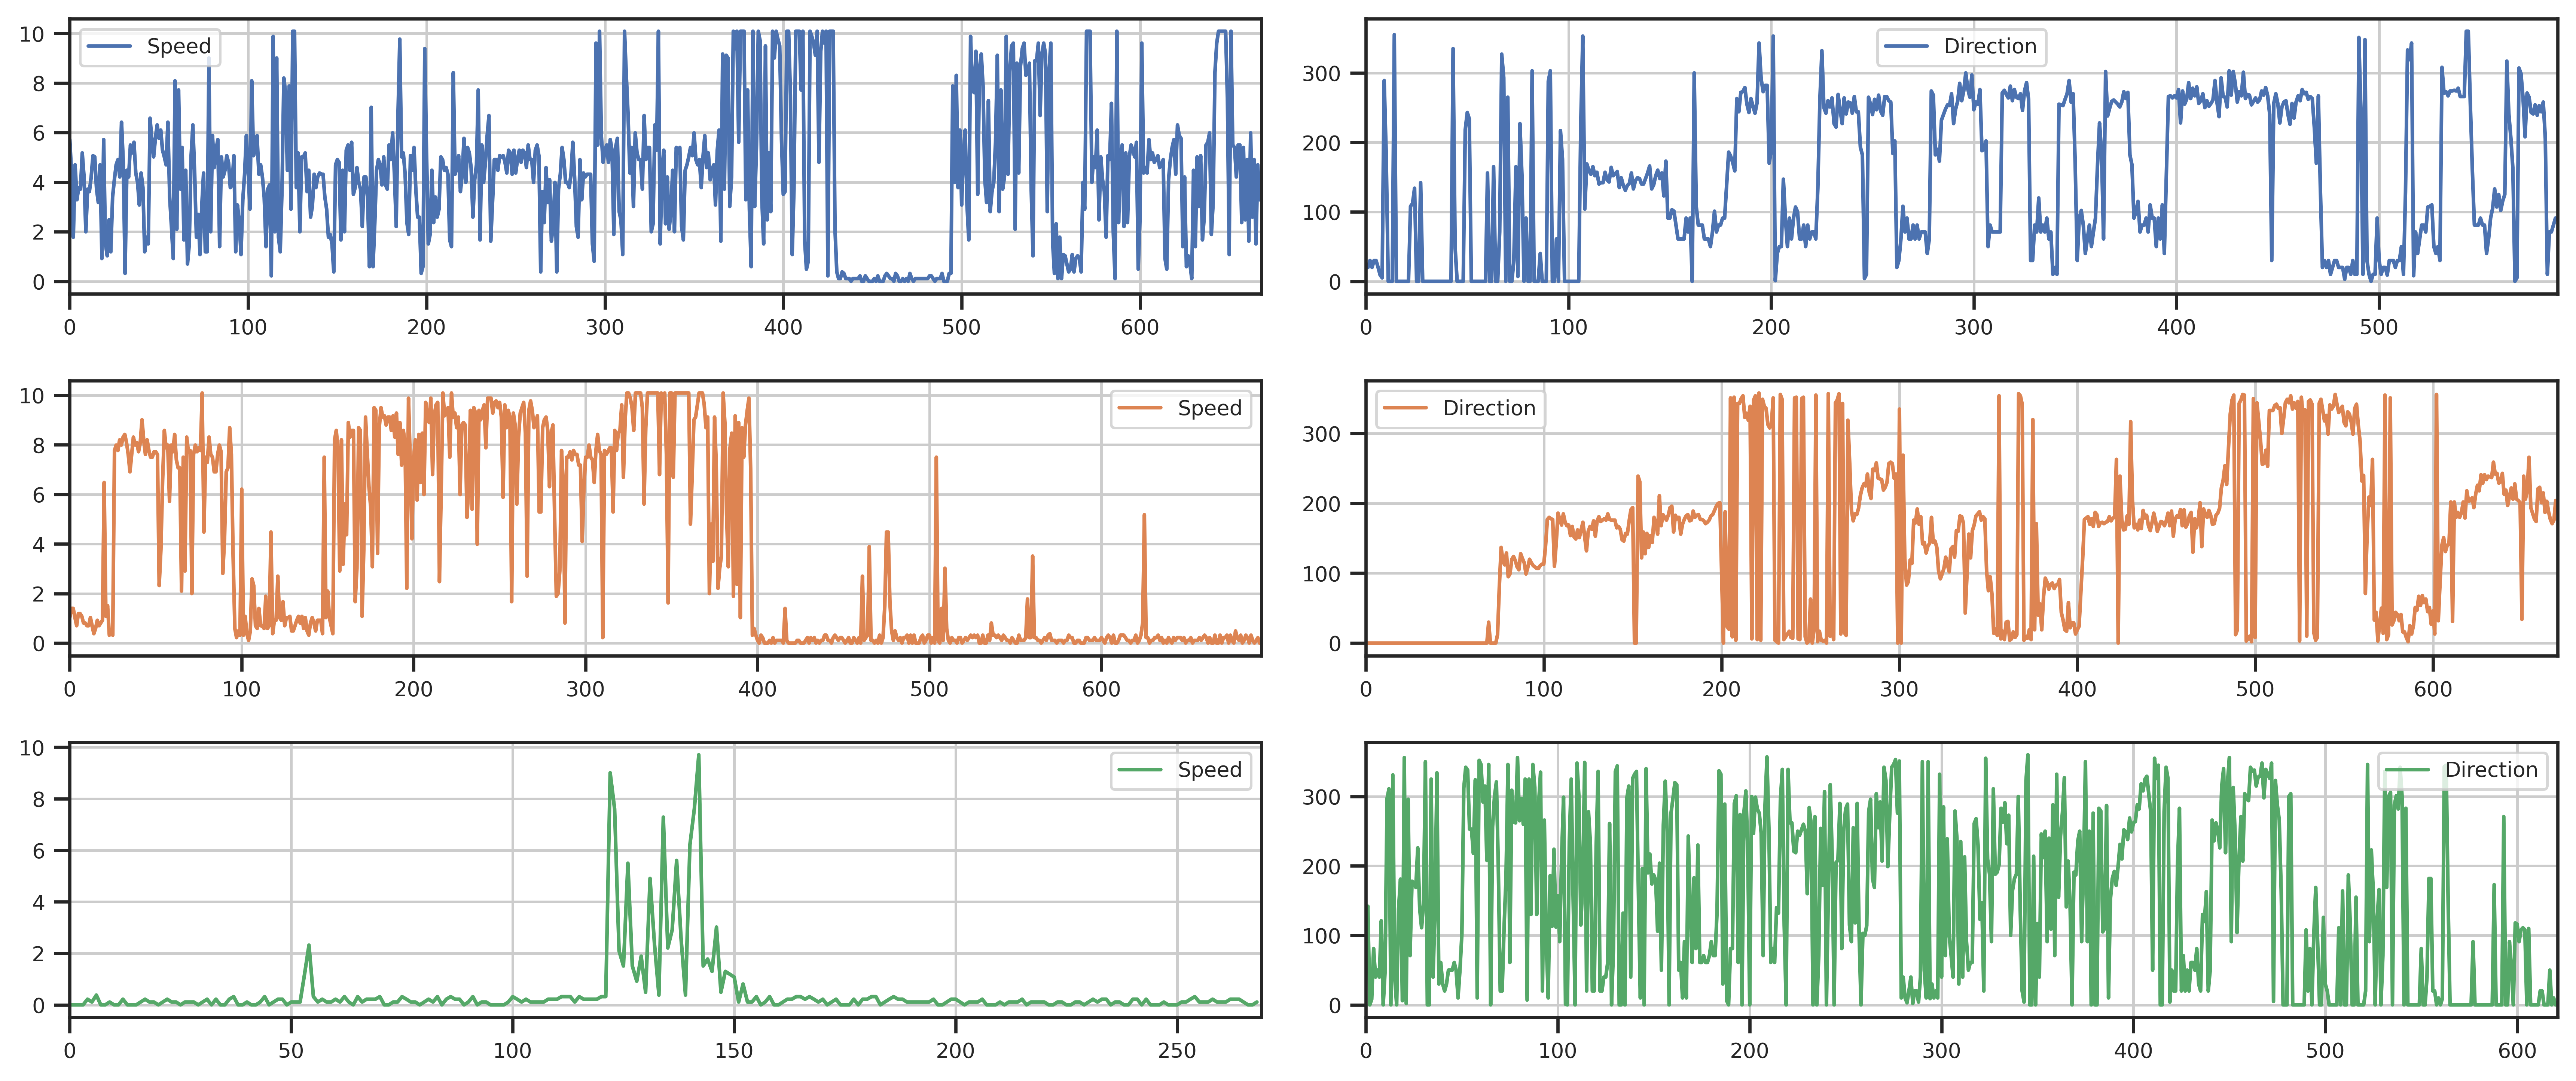
\includegraphics[width=0.75\linewidth]{..//plots//traj_randomly_3_traj_speed_direction.png}
		\caption{不同类别的渔船速度与方向序列信息可视化}
		\label{sec_1_fig_2}
		\vspace{-0.2cm}
	\end{figure}
	进一步绘制三类轨迹的速度序列与方向序列,图(\ref{sec_1_fig_2})为不同作业类别轨迹的速度与方向序列。由图(\ref{sec_1_fig_2})可以得出以下结论:
	\begin{enumerate}
		\item \textbf{轨迹速度数据存在连续低值,强化了POI点存在的判断。}通过图(\ref{sec_1_fig_2})速度序列信息可知,轨迹速度存在连续的速度低值,对于运动目标而言是典型的POI存在的特性。从不同作业类型的渔船的运动特性角度分析,刺网捕捞的渔船更倾向于在同一位置进行捕捞,而拖网与围网类型的轨迹则倾向于有较强的运动性。
		\item \textbf{方向时序振荡显著。}通过多次绘制图(\ref{sec_1_fig_0})可得,方向时间序列振荡明显,不符合正常渔船的运动规律。正常渔船每一次方向的变化,都有较强的目的性,原因在于海上渔船转向或者移动较陆地更为困难,因此方向时序应具有平滑的特性。该情况判断可能是由于船只漂泊造成方向不定。
	\end{enumerate}

	由于不同作业类型的渔船的运动的本质区别,因此,我们采用了类似于针对陆地车辆GPS轨迹的相似的渔船运动模式的建模策略。图(\ref{sec_1_moving_models})为我们的建模策略。事实上,该建模策略主要目的是为了区分渔船的不同的运动模式,从而从特征上更精细的刻画渔船的运动模式。
	\begin{figure}[H]
		\centering
		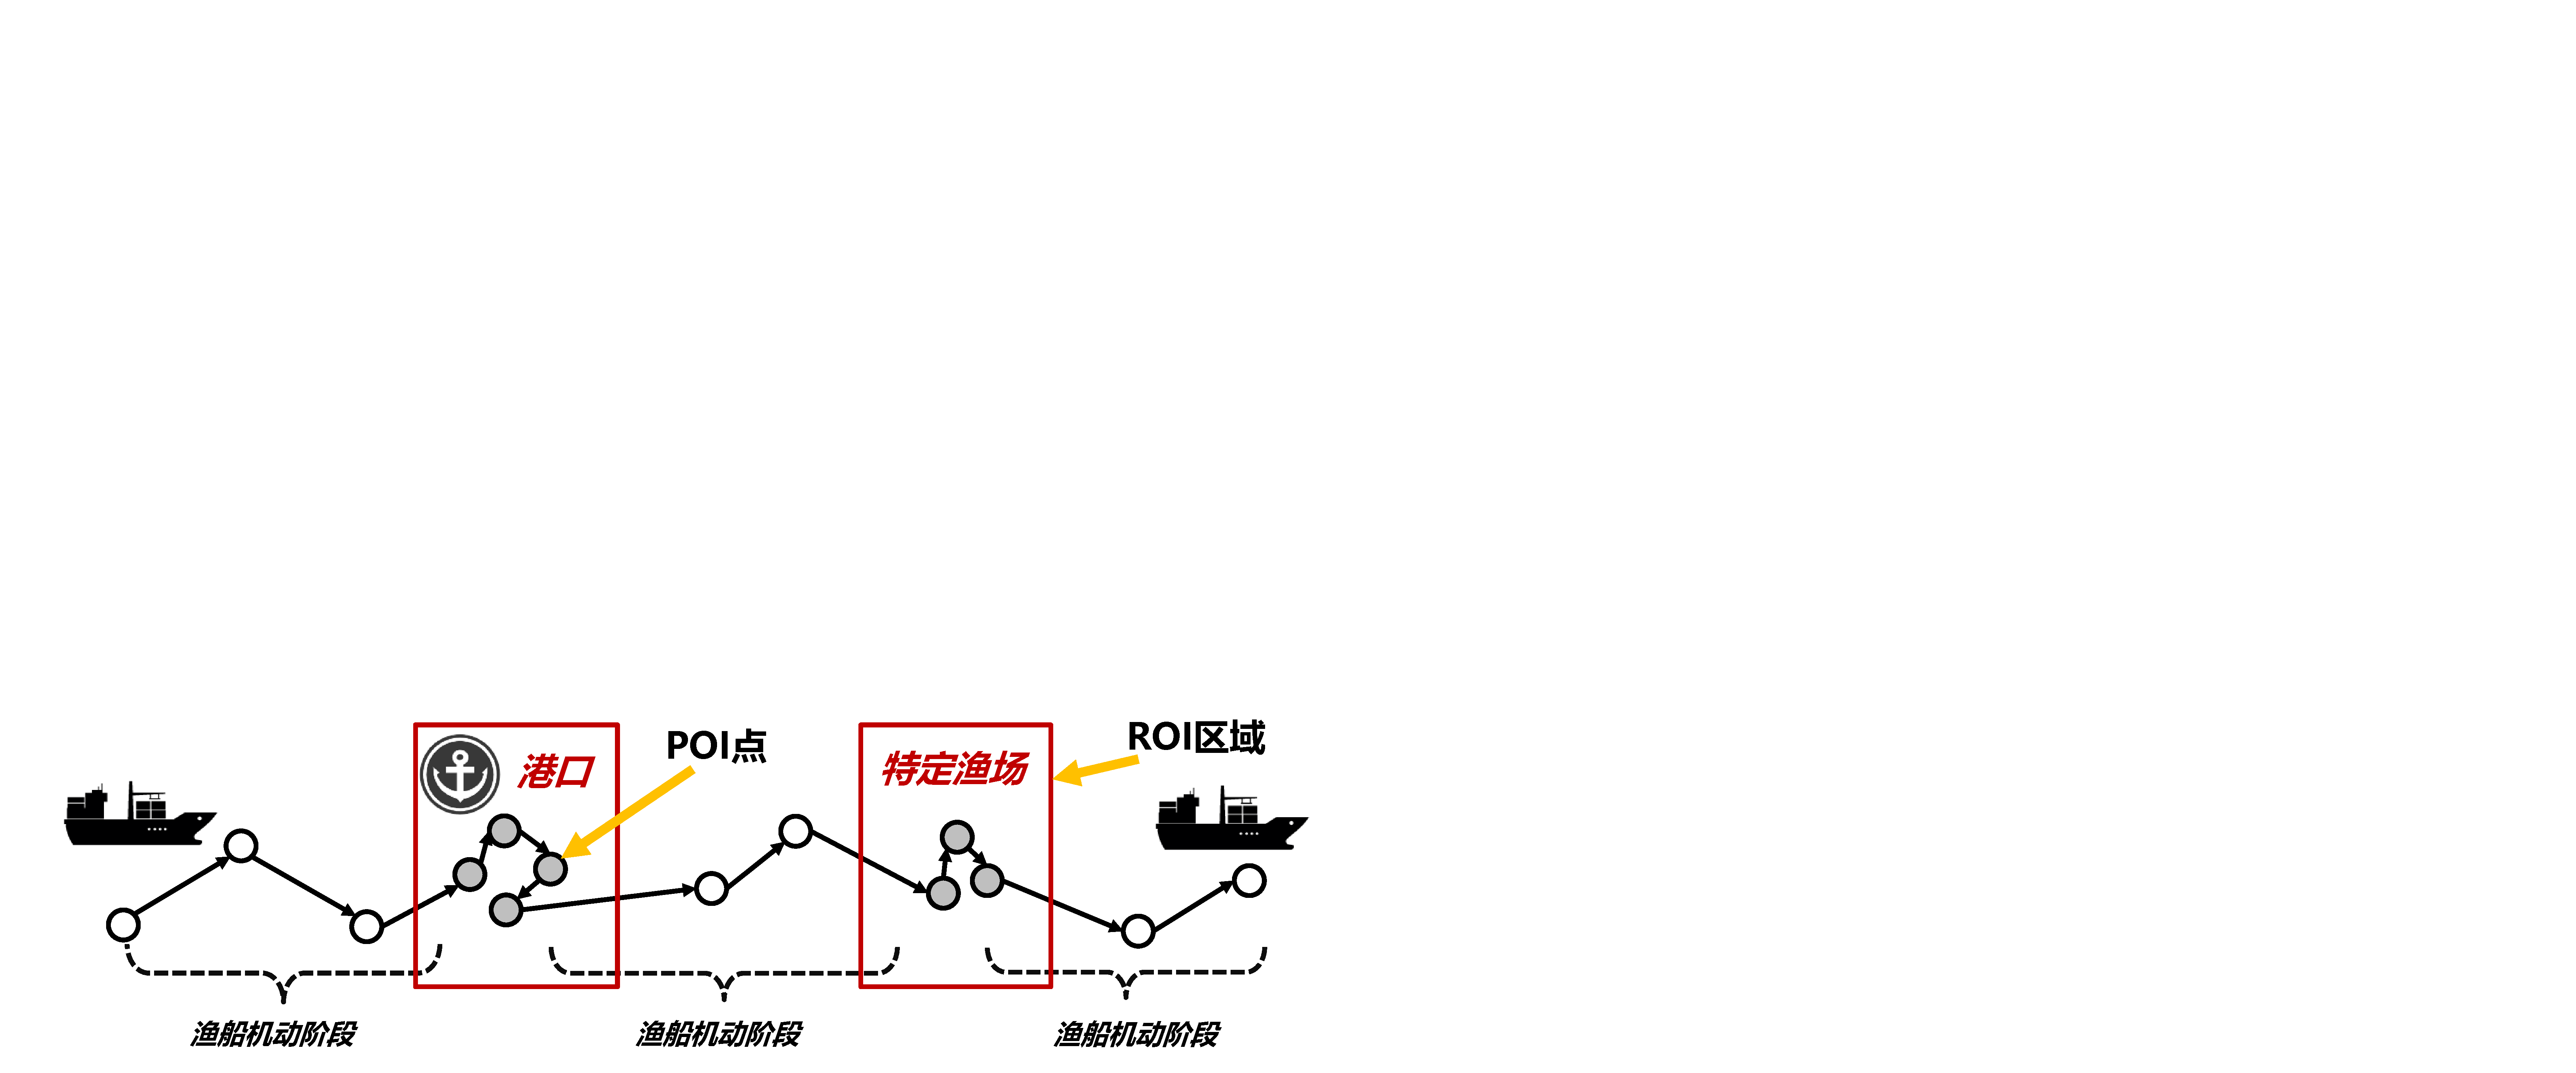
\includegraphics[width=0.75\linewidth]{..//plots//boat_moving_model.pdf}
		\caption{渔船运动模型}
		\label{sec_1_moving_models}
		\vspace{-0.2cm}
	\end{figure}

	在进行基础可视化之后,我们进一步对所有北斗轨迹分布信息进行了可视化分析(注:此处可视化分析已经滤除了少量的影响分布的异常样本,此处意从宏观角度对数据分布进行研究)。
	\begin{figure}[H]
		\centering
		\begin{tabular}{c}
			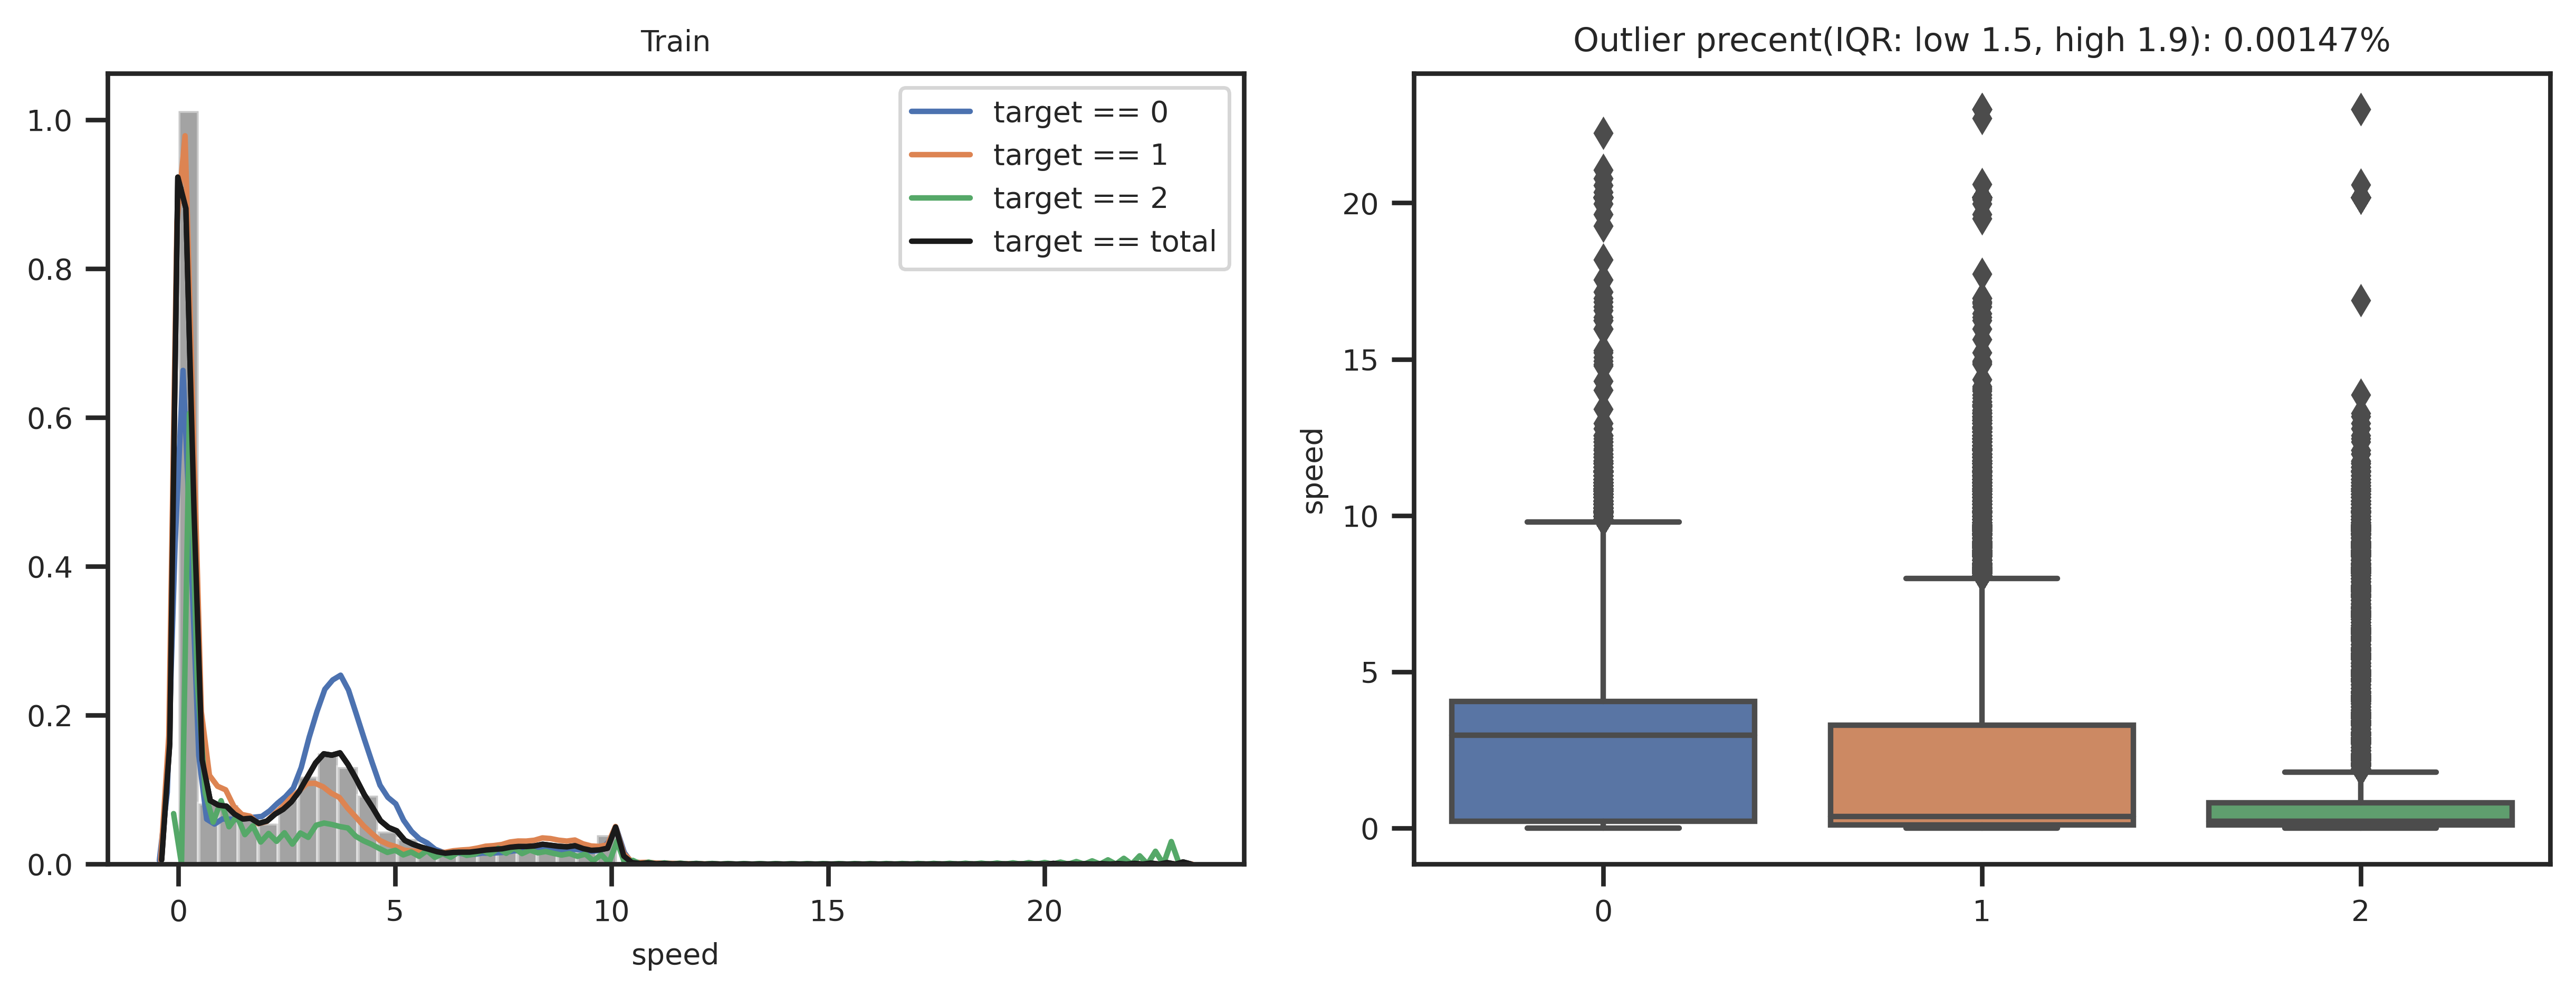
\includegraphics[width=0.65\linewidth]{..//plots//feature_speed_distribution.png} \\
			(a) \\
			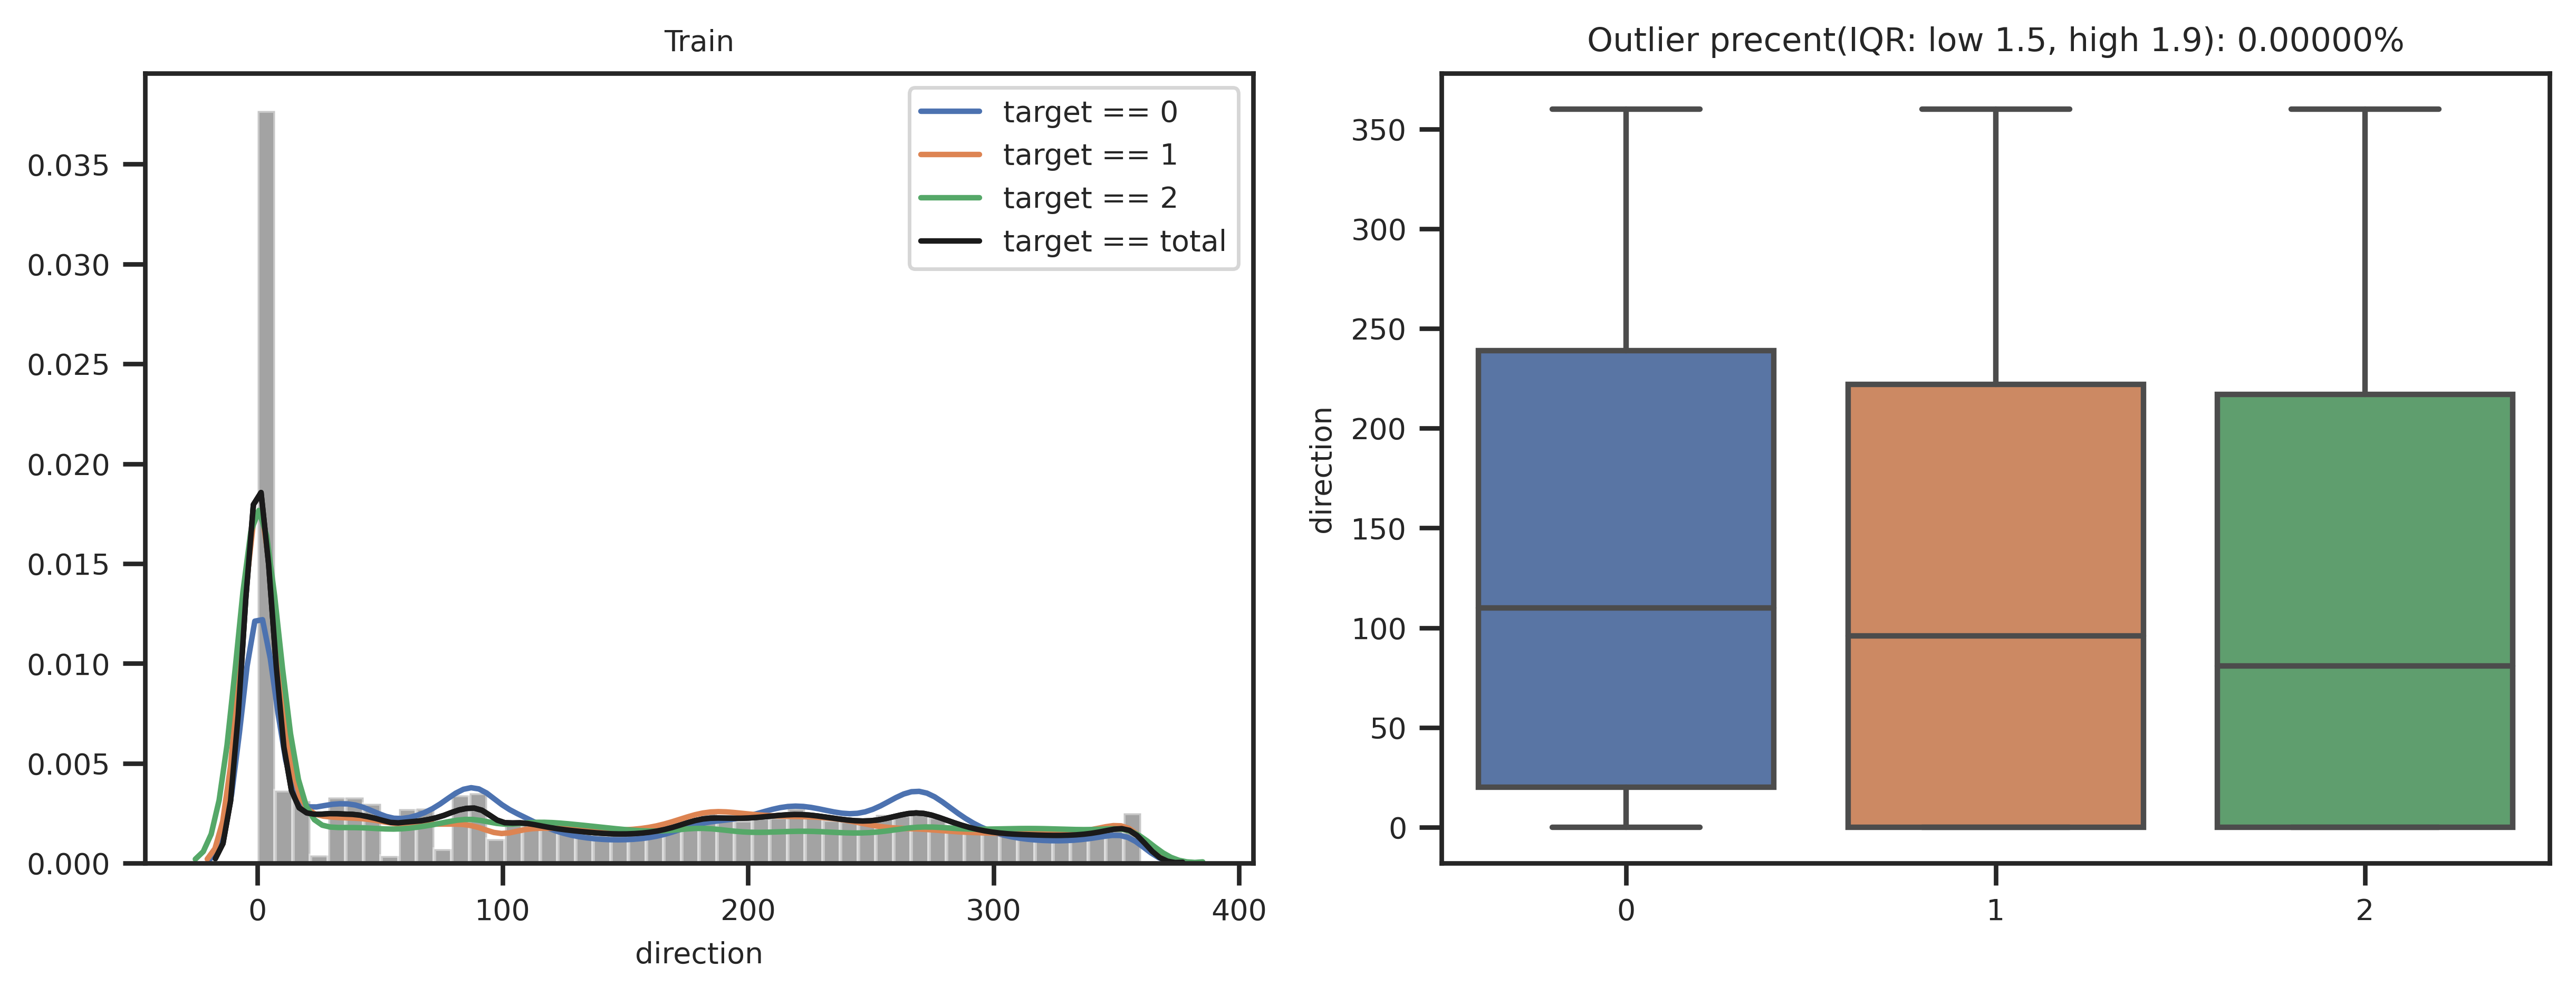
\includegraphics[width=0.65\linewidth]{..//plots//feature_direction_distribution.png} \\
			(b)
		\end{tabular}
		\caption{(a)不同作业类型的轨迹速度分布上的差异; (b)不同作业类别的轨迹方向时序上的分布差异}
		\label{sec_1_fig_3}
		\vspace{-0.2cm}
	\end{figure}
	图(\ref{sec_1_fig_3})为我们将所有轨迹拼接起来(Concat)后,不同作业类别的轨迹速度与方向的分布特征与箱型图。由图(\ref{sec_1_fig_3})可知:
	\begin{enumerate}
		\item \textbf{轨迹速度数据存在噪声。}即使在对每条轨迹的速度时序进行平滑之后,发现仍然轨迹中存在有大量离群点,说明速度信息中存在噪声。
		\item \textbf{不同类别的渔船,速度整体分布上存在差异。}通过图(\ref{sec_1_fig_3})的(a)图可以看出,不同作业类型的渔船,分布上存在一些差异。分位数特征能够捕获这样的差异。
		\item \textbf{不同捕捞行为的渔船, 方向分布特征不明显。}图(\ref{sec_1_fig_3})的(b)图可知,方向分布特征并不能很好的区分不同类别的渔船。
	\end{enumerate}

	在有了上述第2点的结论之后,我们进一步对不同作业类别的渔船的速度分布和方向分布特征进行了可视化分析。
	\begin{figure}[H]
		\centering
		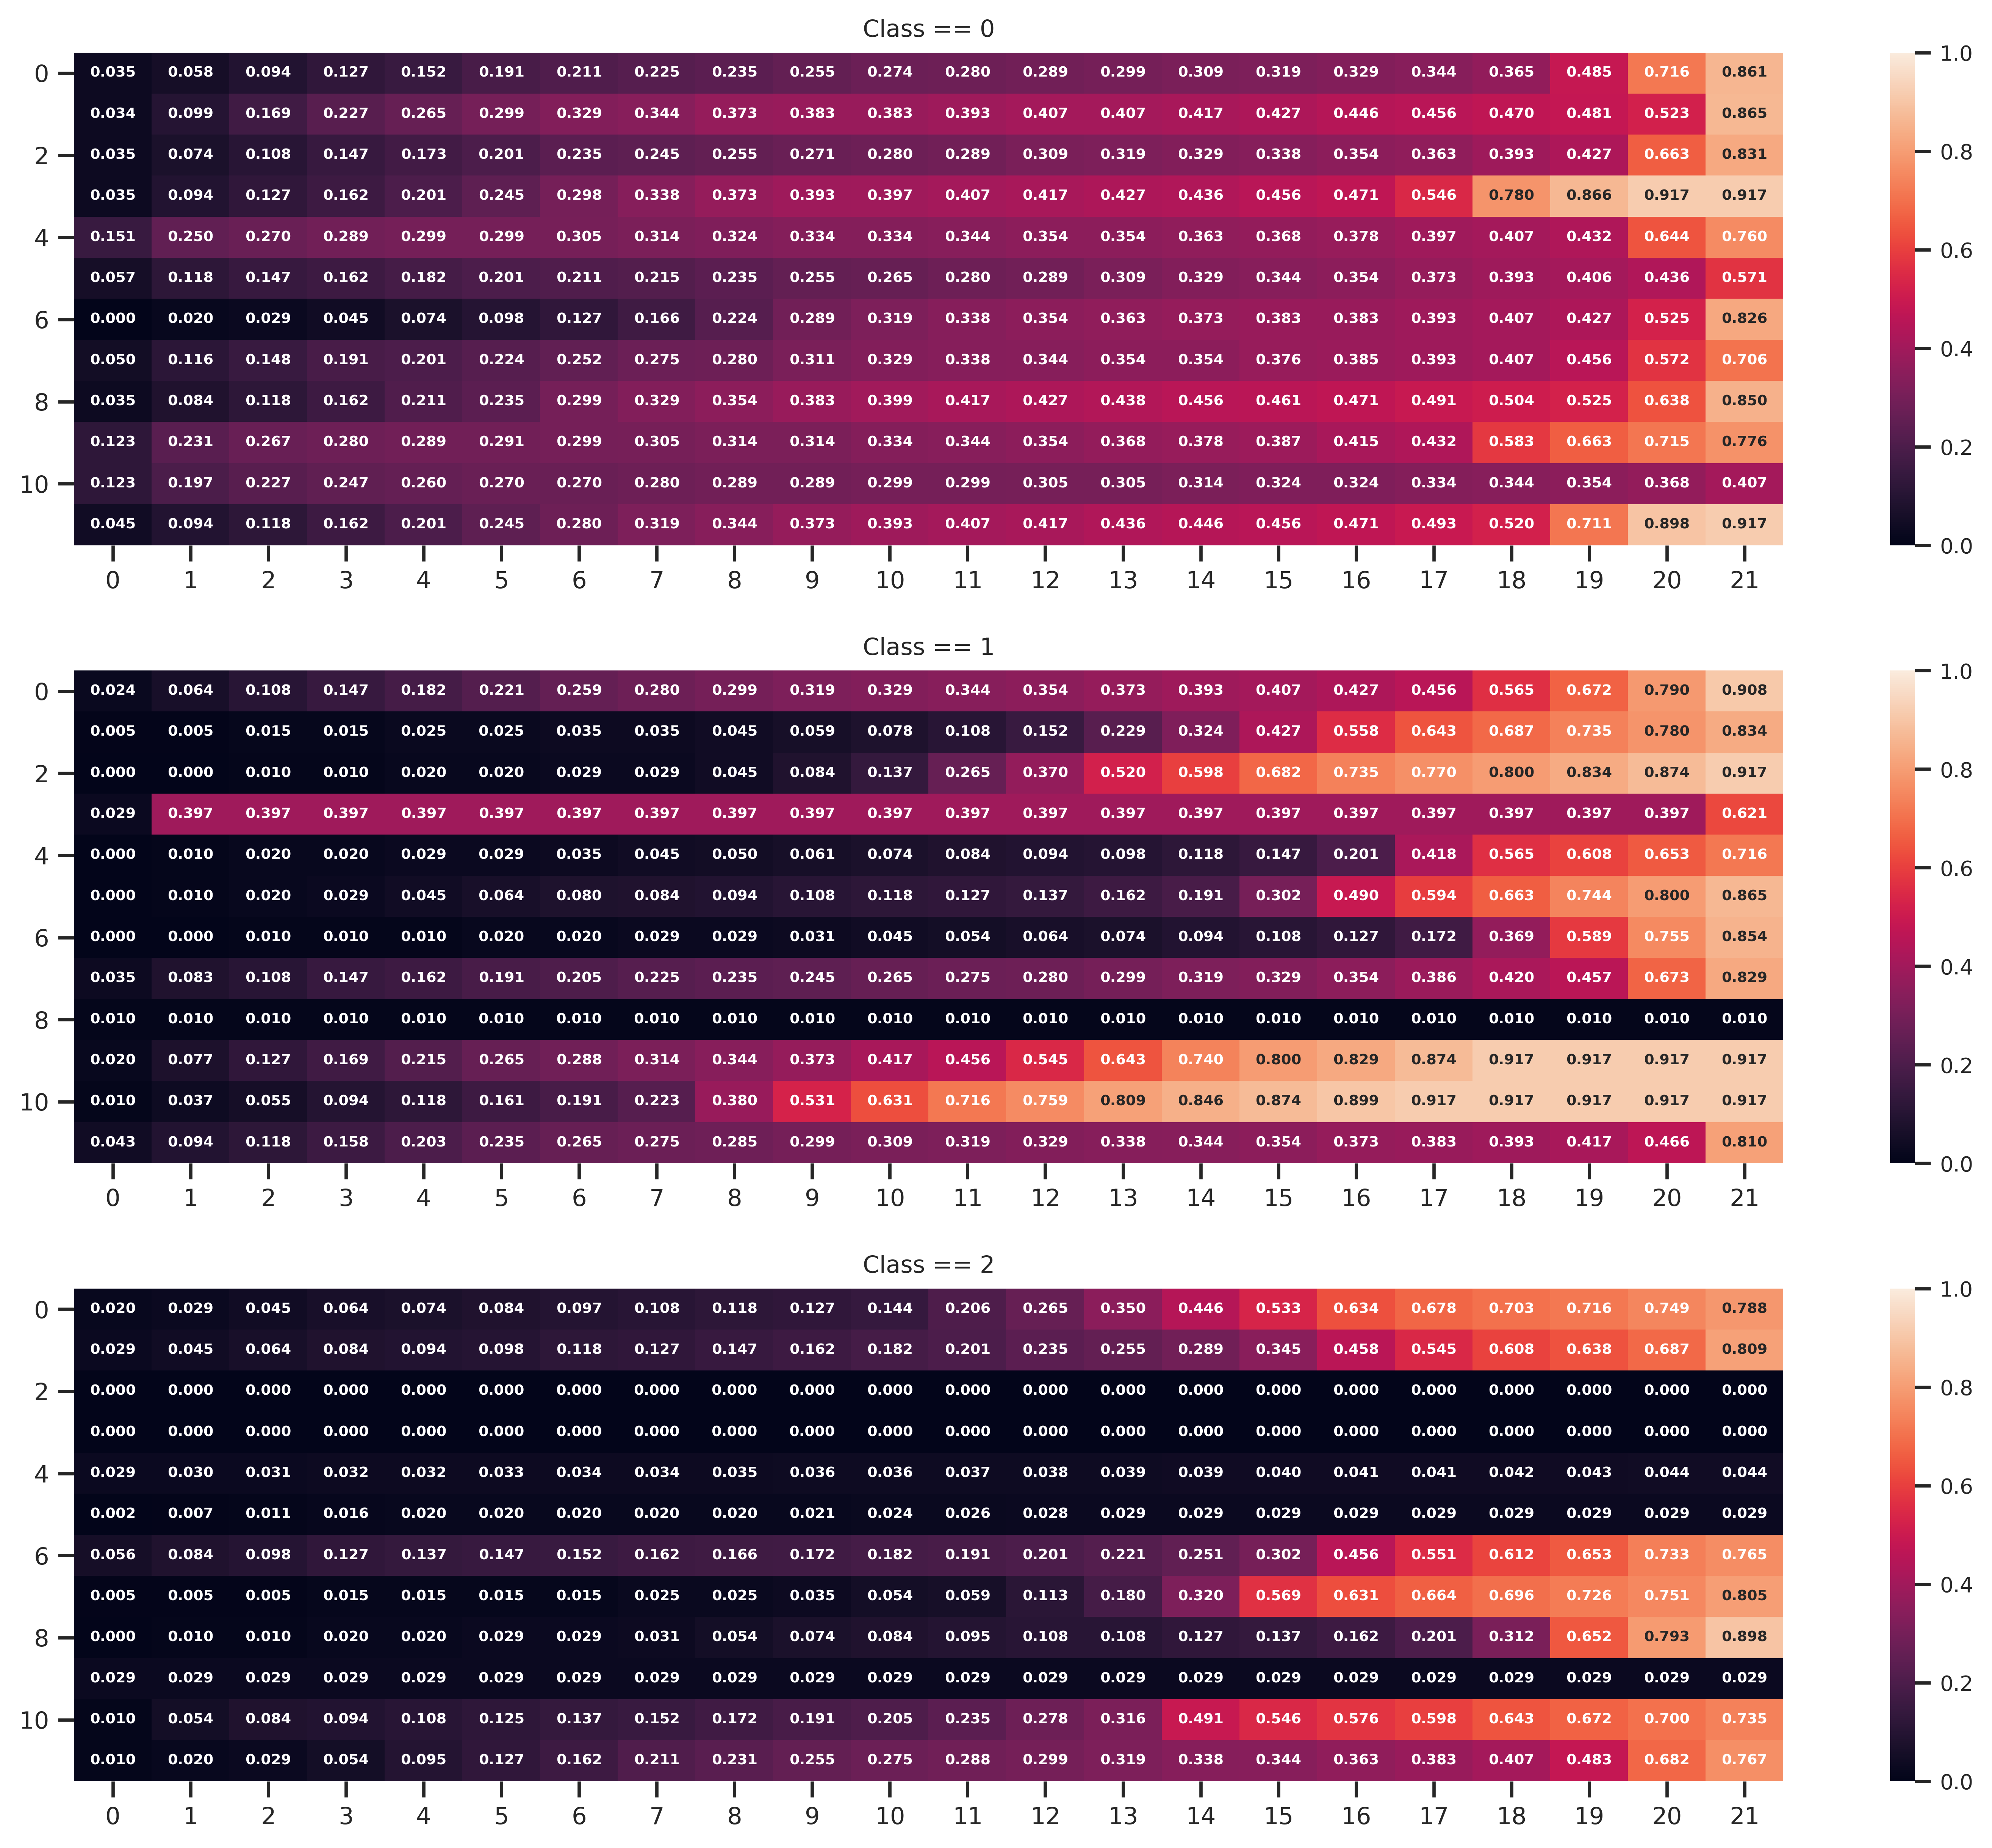
\includegraphics[width=0.45\linewidth]{..//plots//feature_speed_quantile_heatmap.png}
		\caption{不同作业类型的渔船速度分位数热力图}
		\label{sec_1_fig_4}
		\vspace{-0.2cm}
	\end{figure}
	图(\ref{sec_1_fig_4})为不同作业类型的渔船随机挑选出一些样本抽取其速度的分位数获得获得的热力图(数值已事先归一化)。由图(\ref{sec_1_fig_4})可以看出不同类别渔船速度分布确实有较强的差异性,尤其是Class 0(拖网)与Class 1(围网)和Class 2(刺网)之间差异较为明显。这也与拖网渔船长期拖网捕捞的运动特性有很强的联系。事实上速度分位数特征也是后续机器学习模型的强特。

	图(\ref{sec_1_fig_5})为不同作业类型的渔船随机挑选出一些样本抽取其方向序列的分位数获得获得的热力图(数值已事先归一化)。
	\begin{figure}[H]
		\centering
		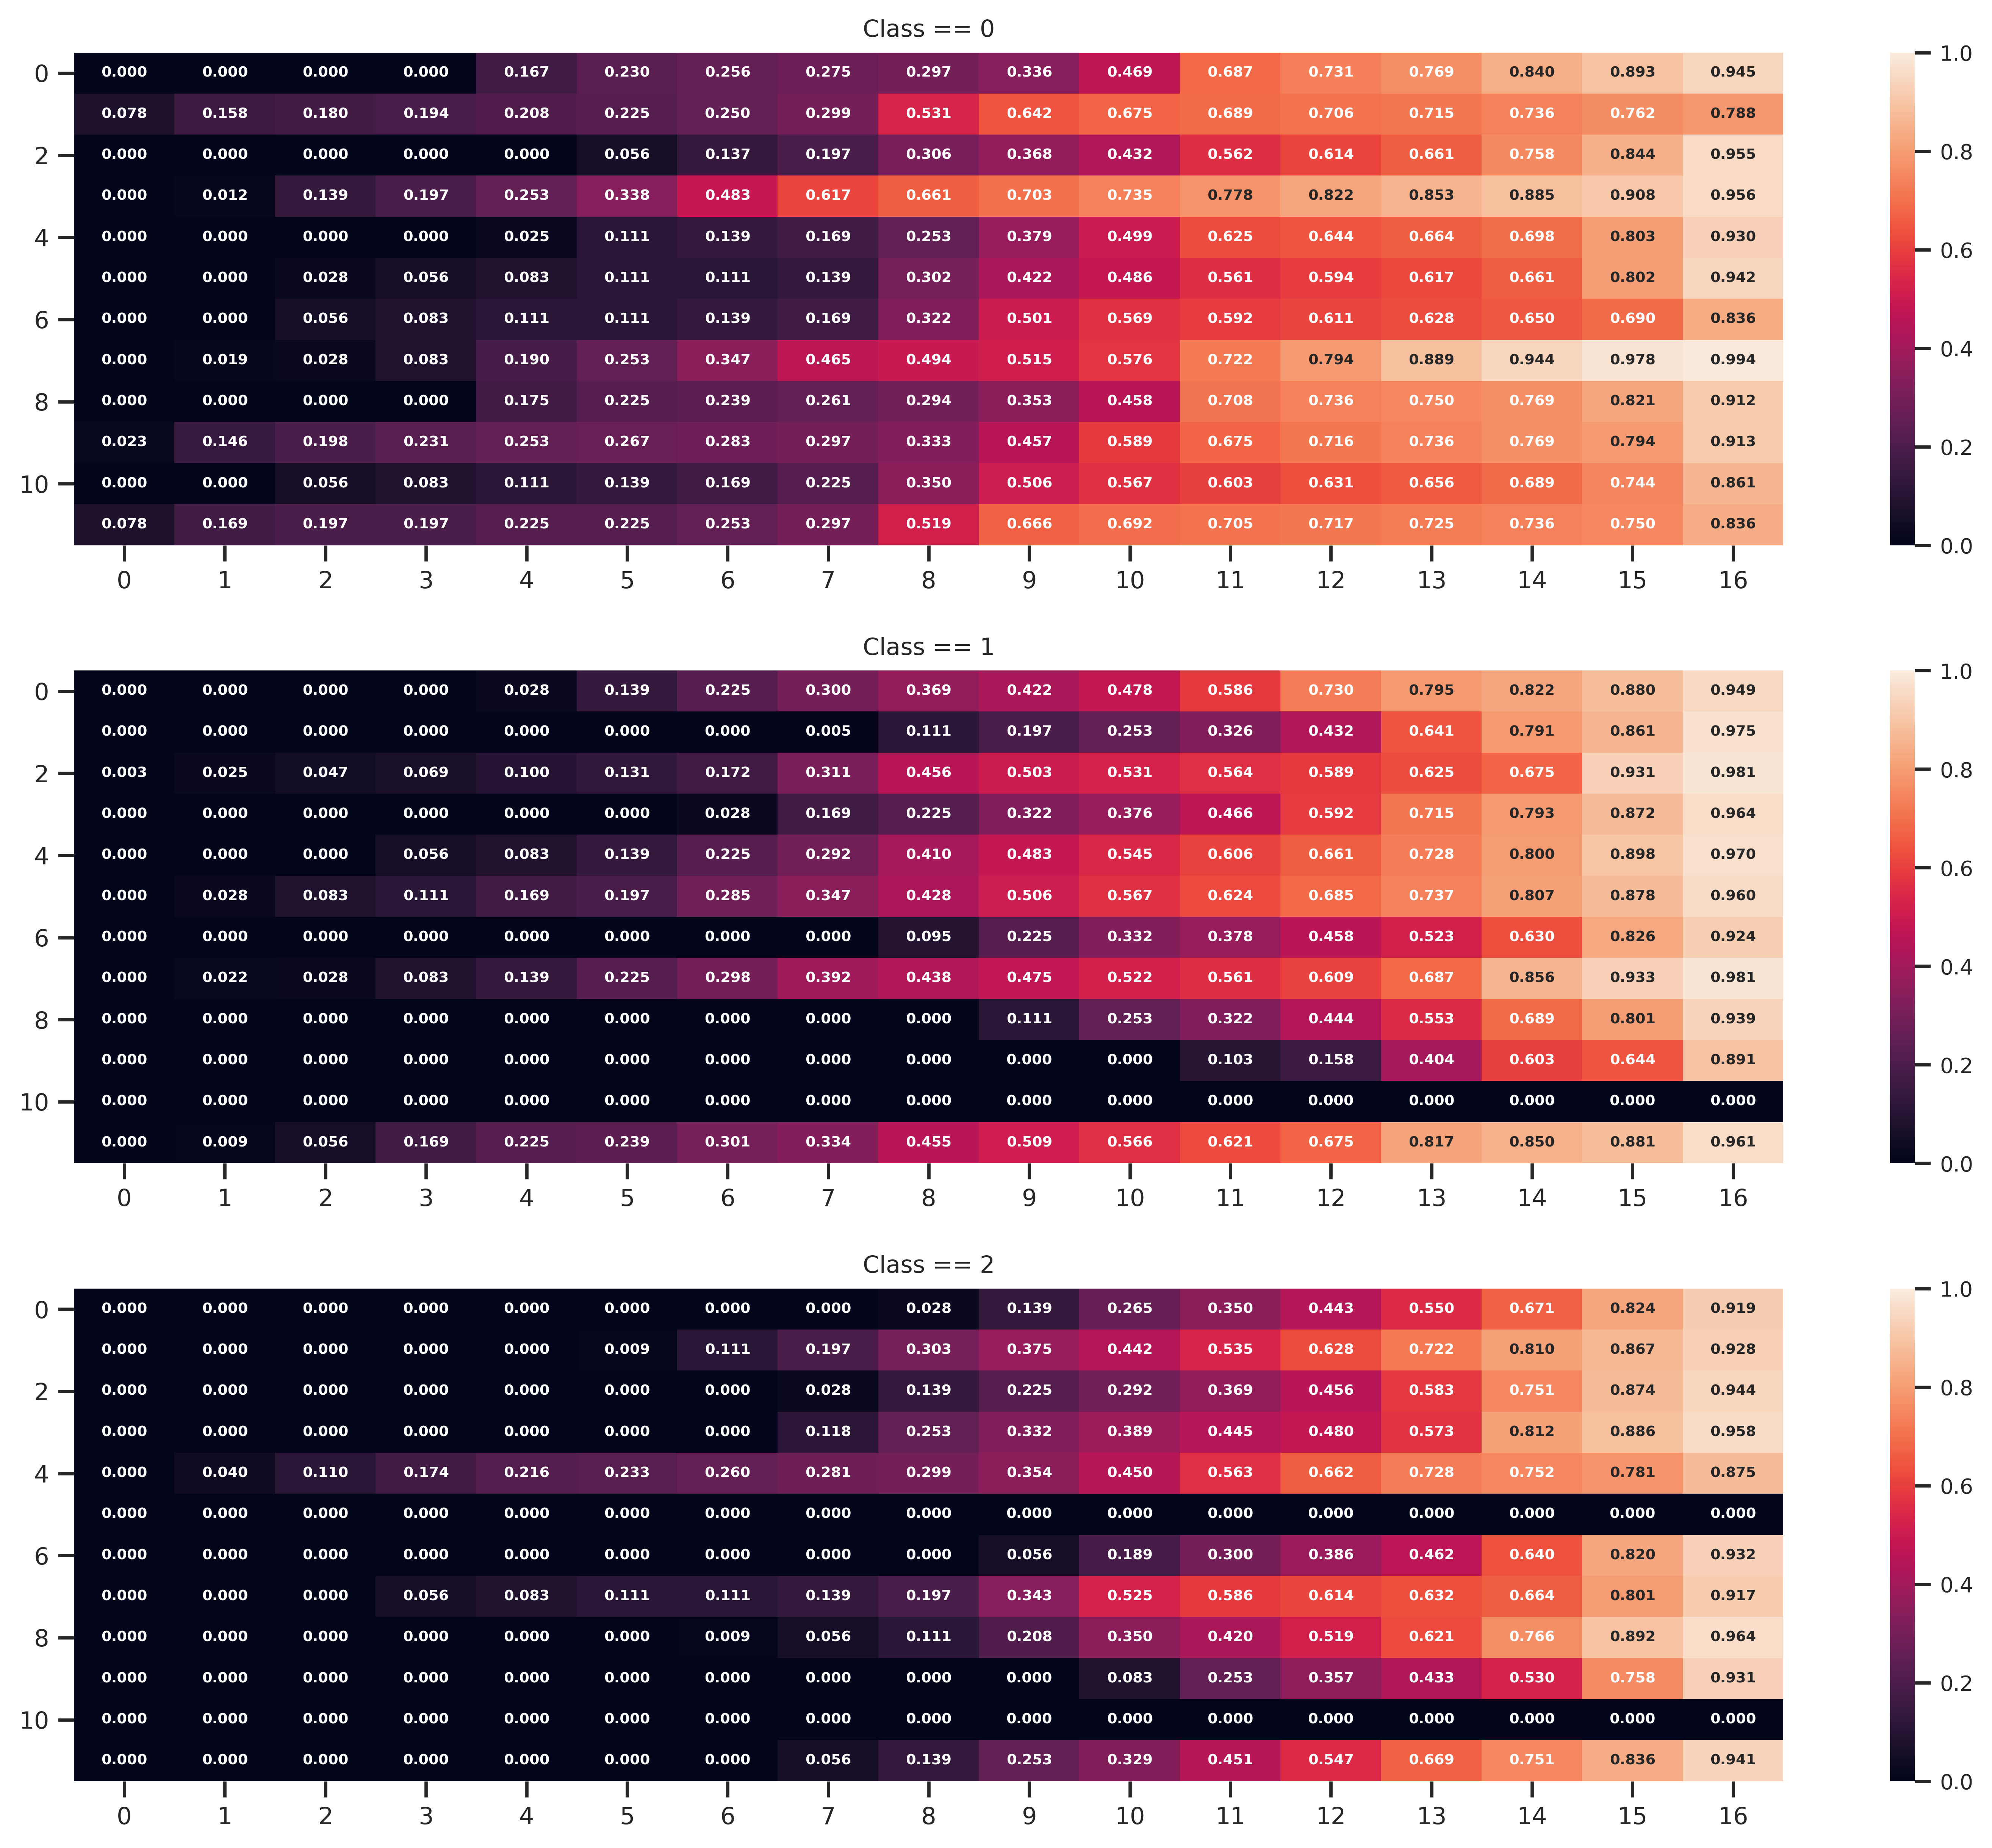
\includegraphics[width=0.45\linewidth]{..//plots//feature_dir_quantile_heatmap.png}
		\caption{不同作业类型的渔船方向分位数热力图}
		\label{sec_1_fig_5}
		\vspace{-0.2cm}
	\end{figure}
	从方向热力图上,并不能直观看出不同类别轨迹之间的差异。后期经过实践,方向特征确实没有发挥太大的作用。

	在分析了速度与方向的分布特征之后,我们进一步分析了每条轨迹的经度与纬度的总体分布特征。一般来说在移动数据挖掘中,不同经纬度的地点往往具有很强的语义信息,对模型的构建至关重要。图(\ref{sec_1_fig_6})为我们将所有轨迹拼接起来(Concat)后,不同作业类别的轨迹经度与纬度的分布特征与箱型图。
	\begin{figure}[H]
		\centering
		\begin{tabular}{c}
			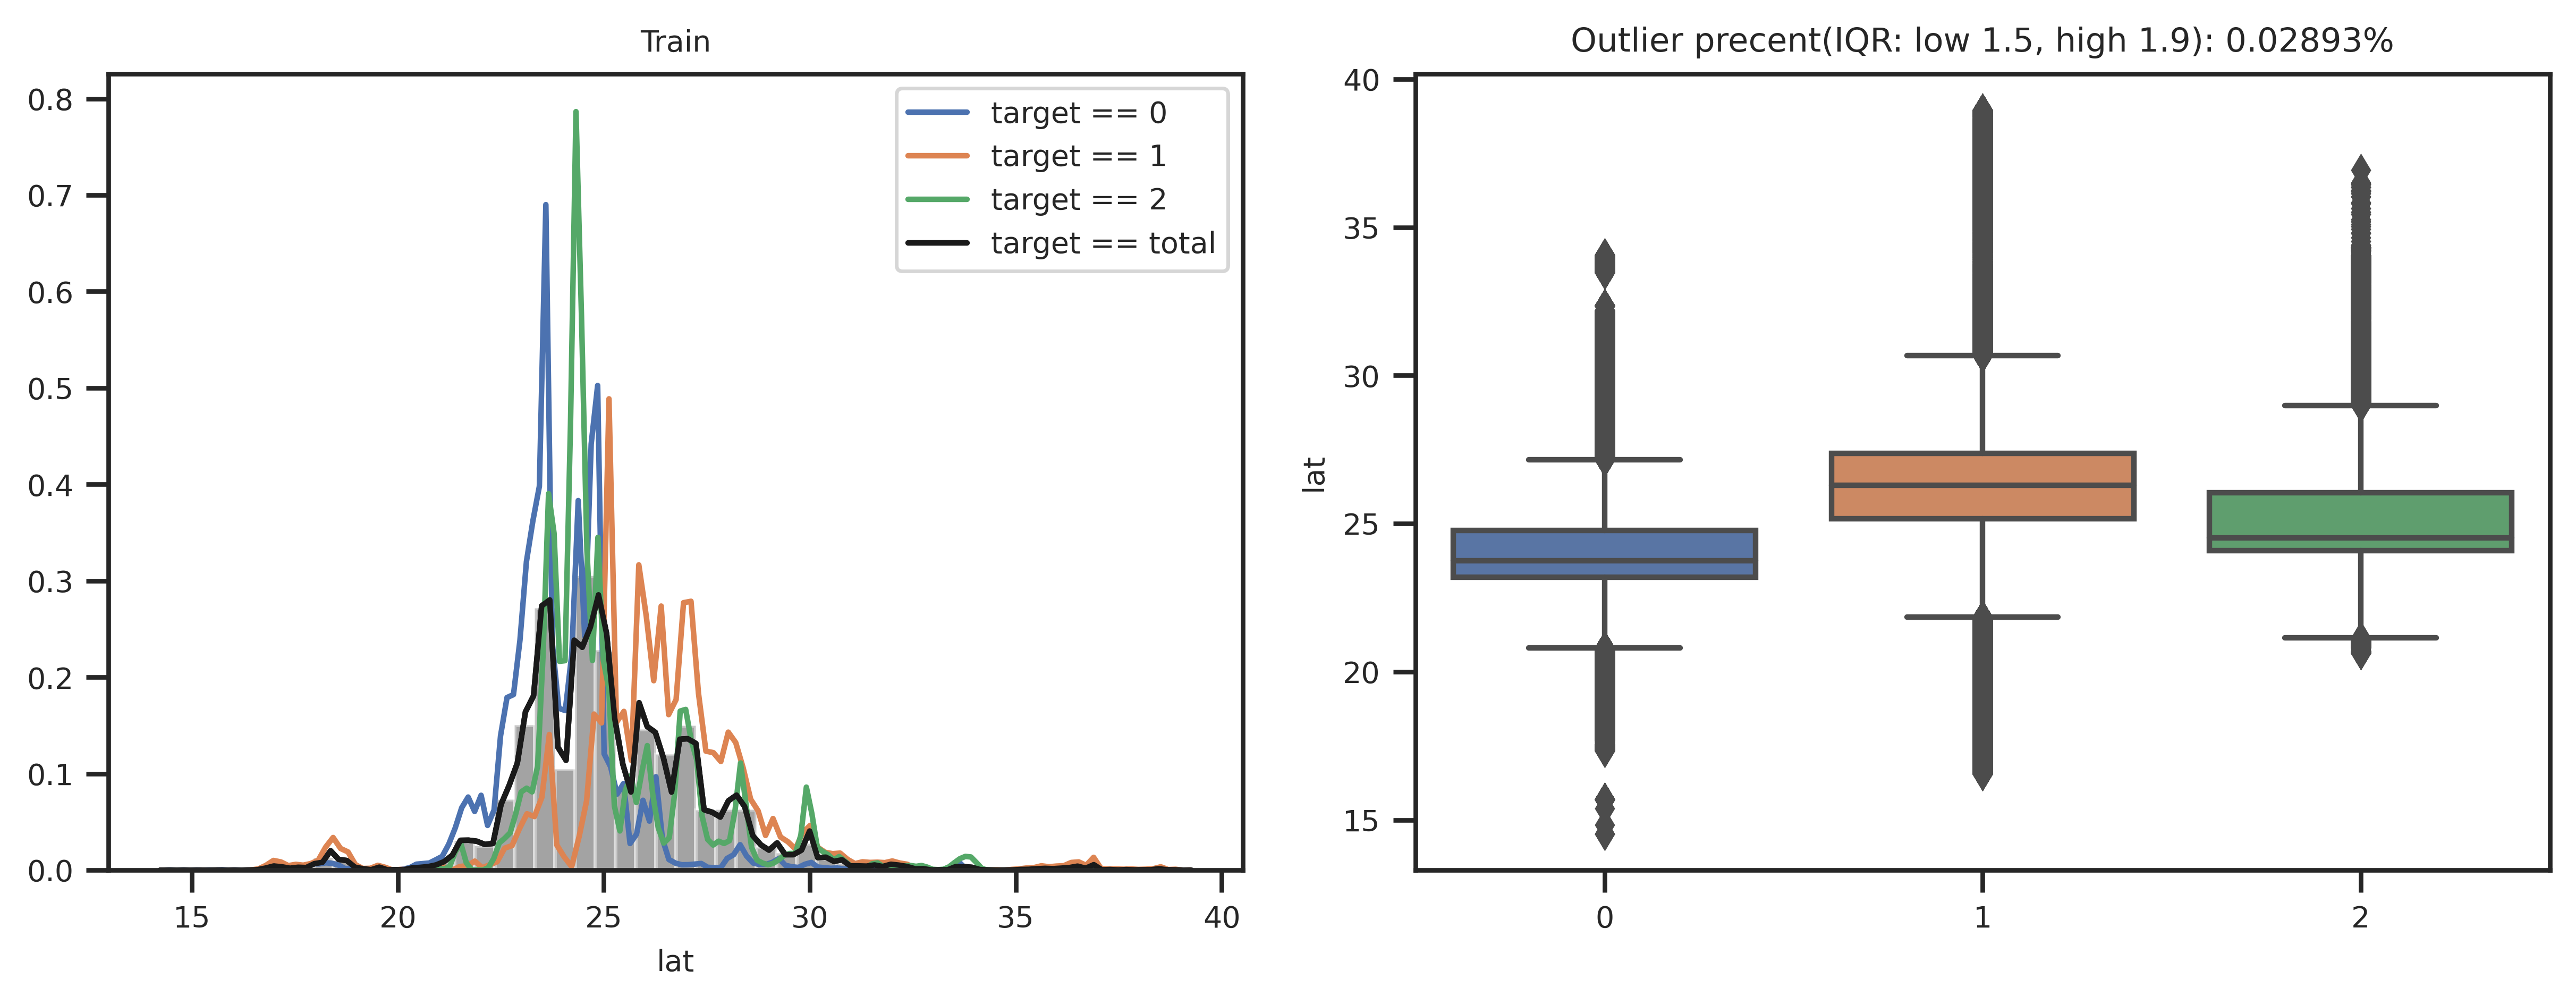
\includegraphics[width=0.75\linewidth]{..//plots//feature_lat_distribution.png} \\
			(a) \\
			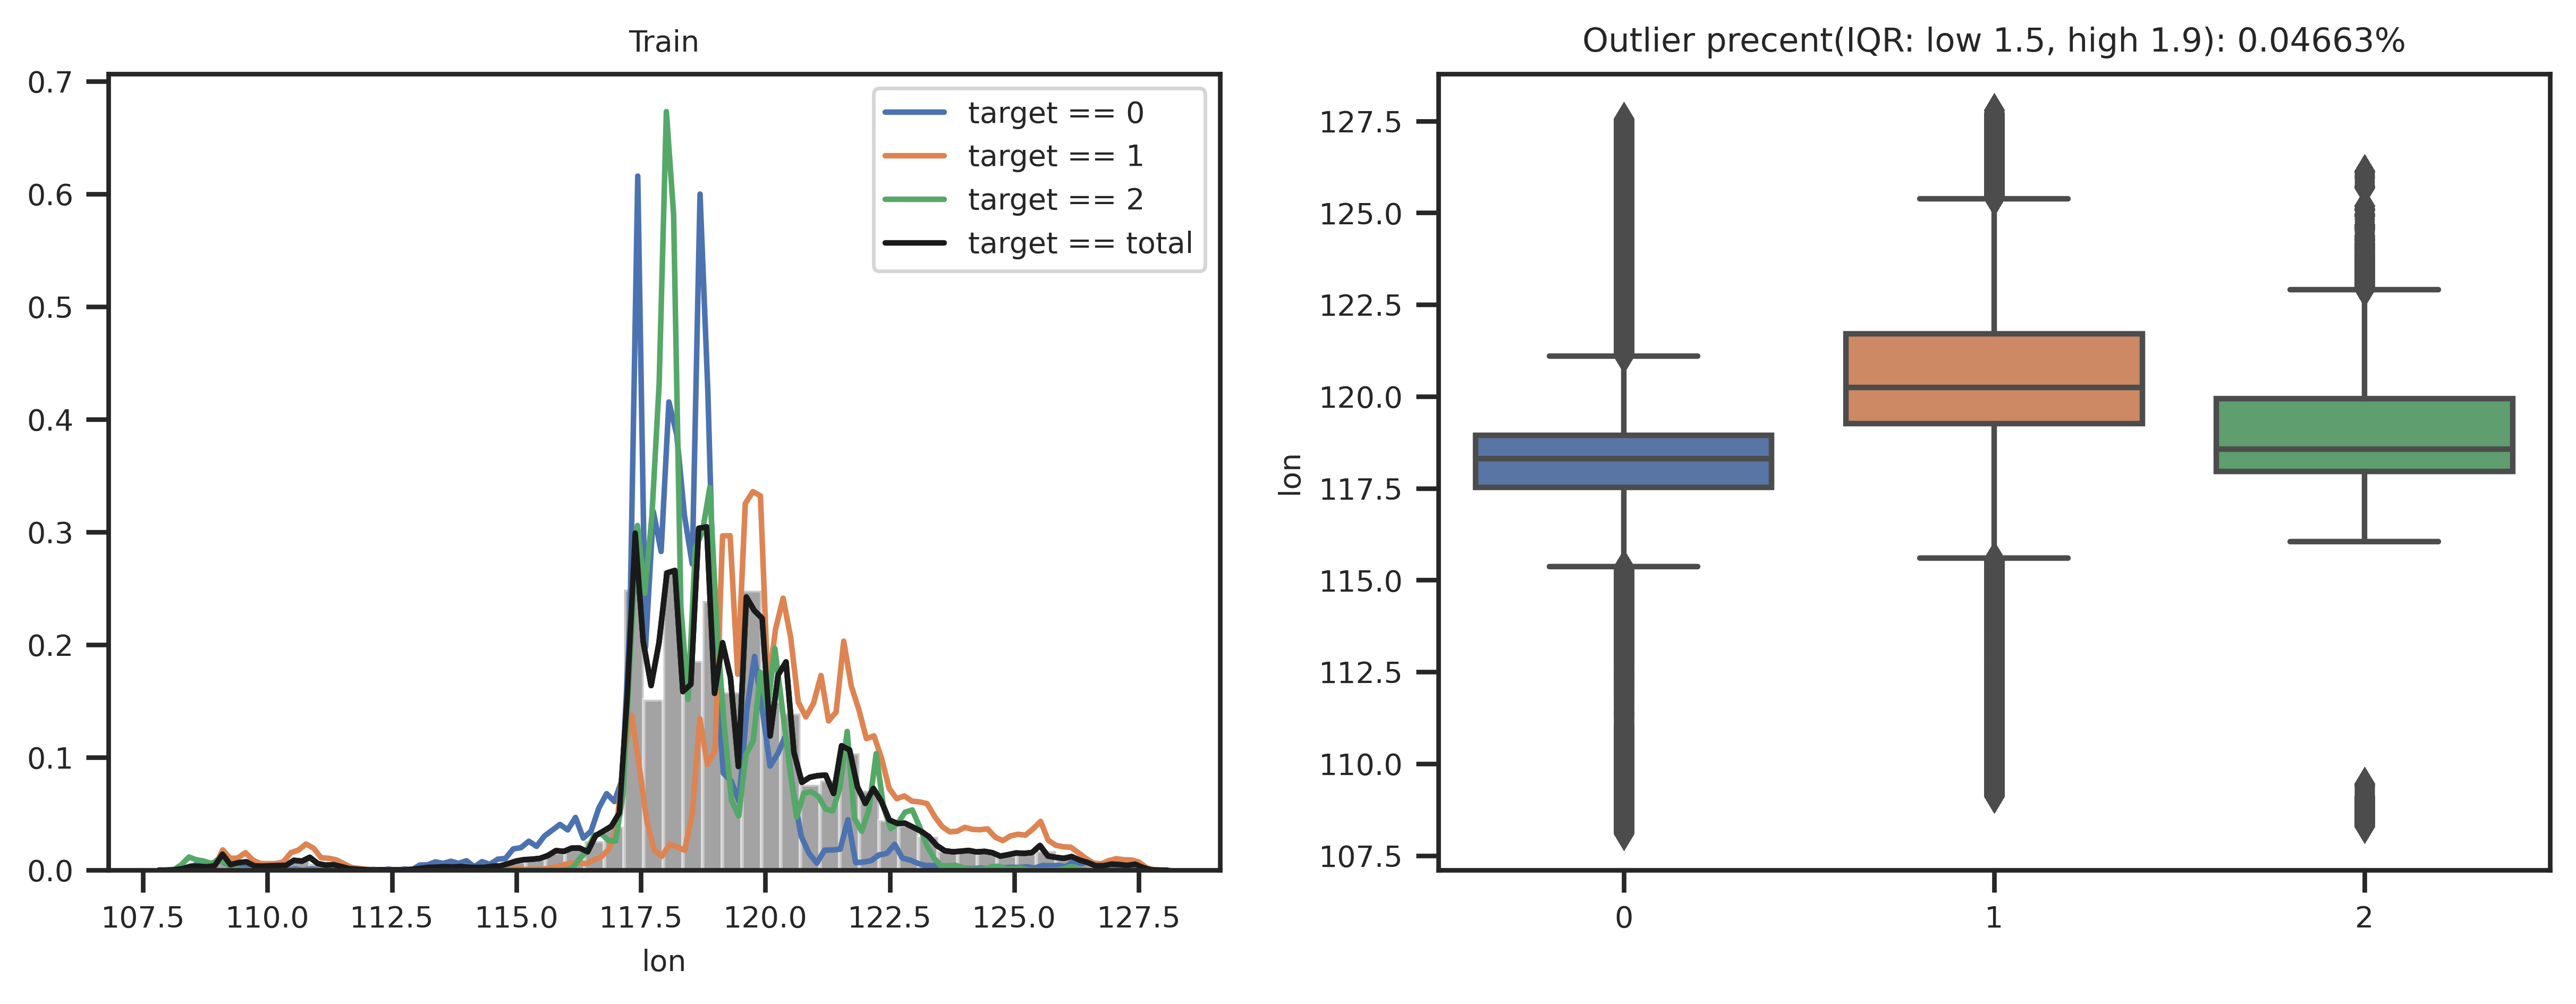
\includegraphics[width=0.75\linewidth]{..//plots//feature_lon_distribution.png} \\
			(b)
		\end{tabular}
		\caption{(a)不同作业类型的轨迹经度分布上的差异; (b)不同作业类别的轨迹纬度的分布差异}
		\label{sec_1_fig_6}
		\vspace{-0.2cm}
	\end{figure}
	由图(\ref{sec_1_fig_6})可以看出,不同作业类型的渔船经纬度分布上有着明显的差异。同样可以使用分位数特征来捕获这样的分布差异。同时,我们对每一条轨迹计算了其平均坐标与最频繁的坐标,并在地图上进行了可视化。图(\ref{sec_1_fig_7})为坐标可视化效果。
	\begin{figure}[H]
		\centering
		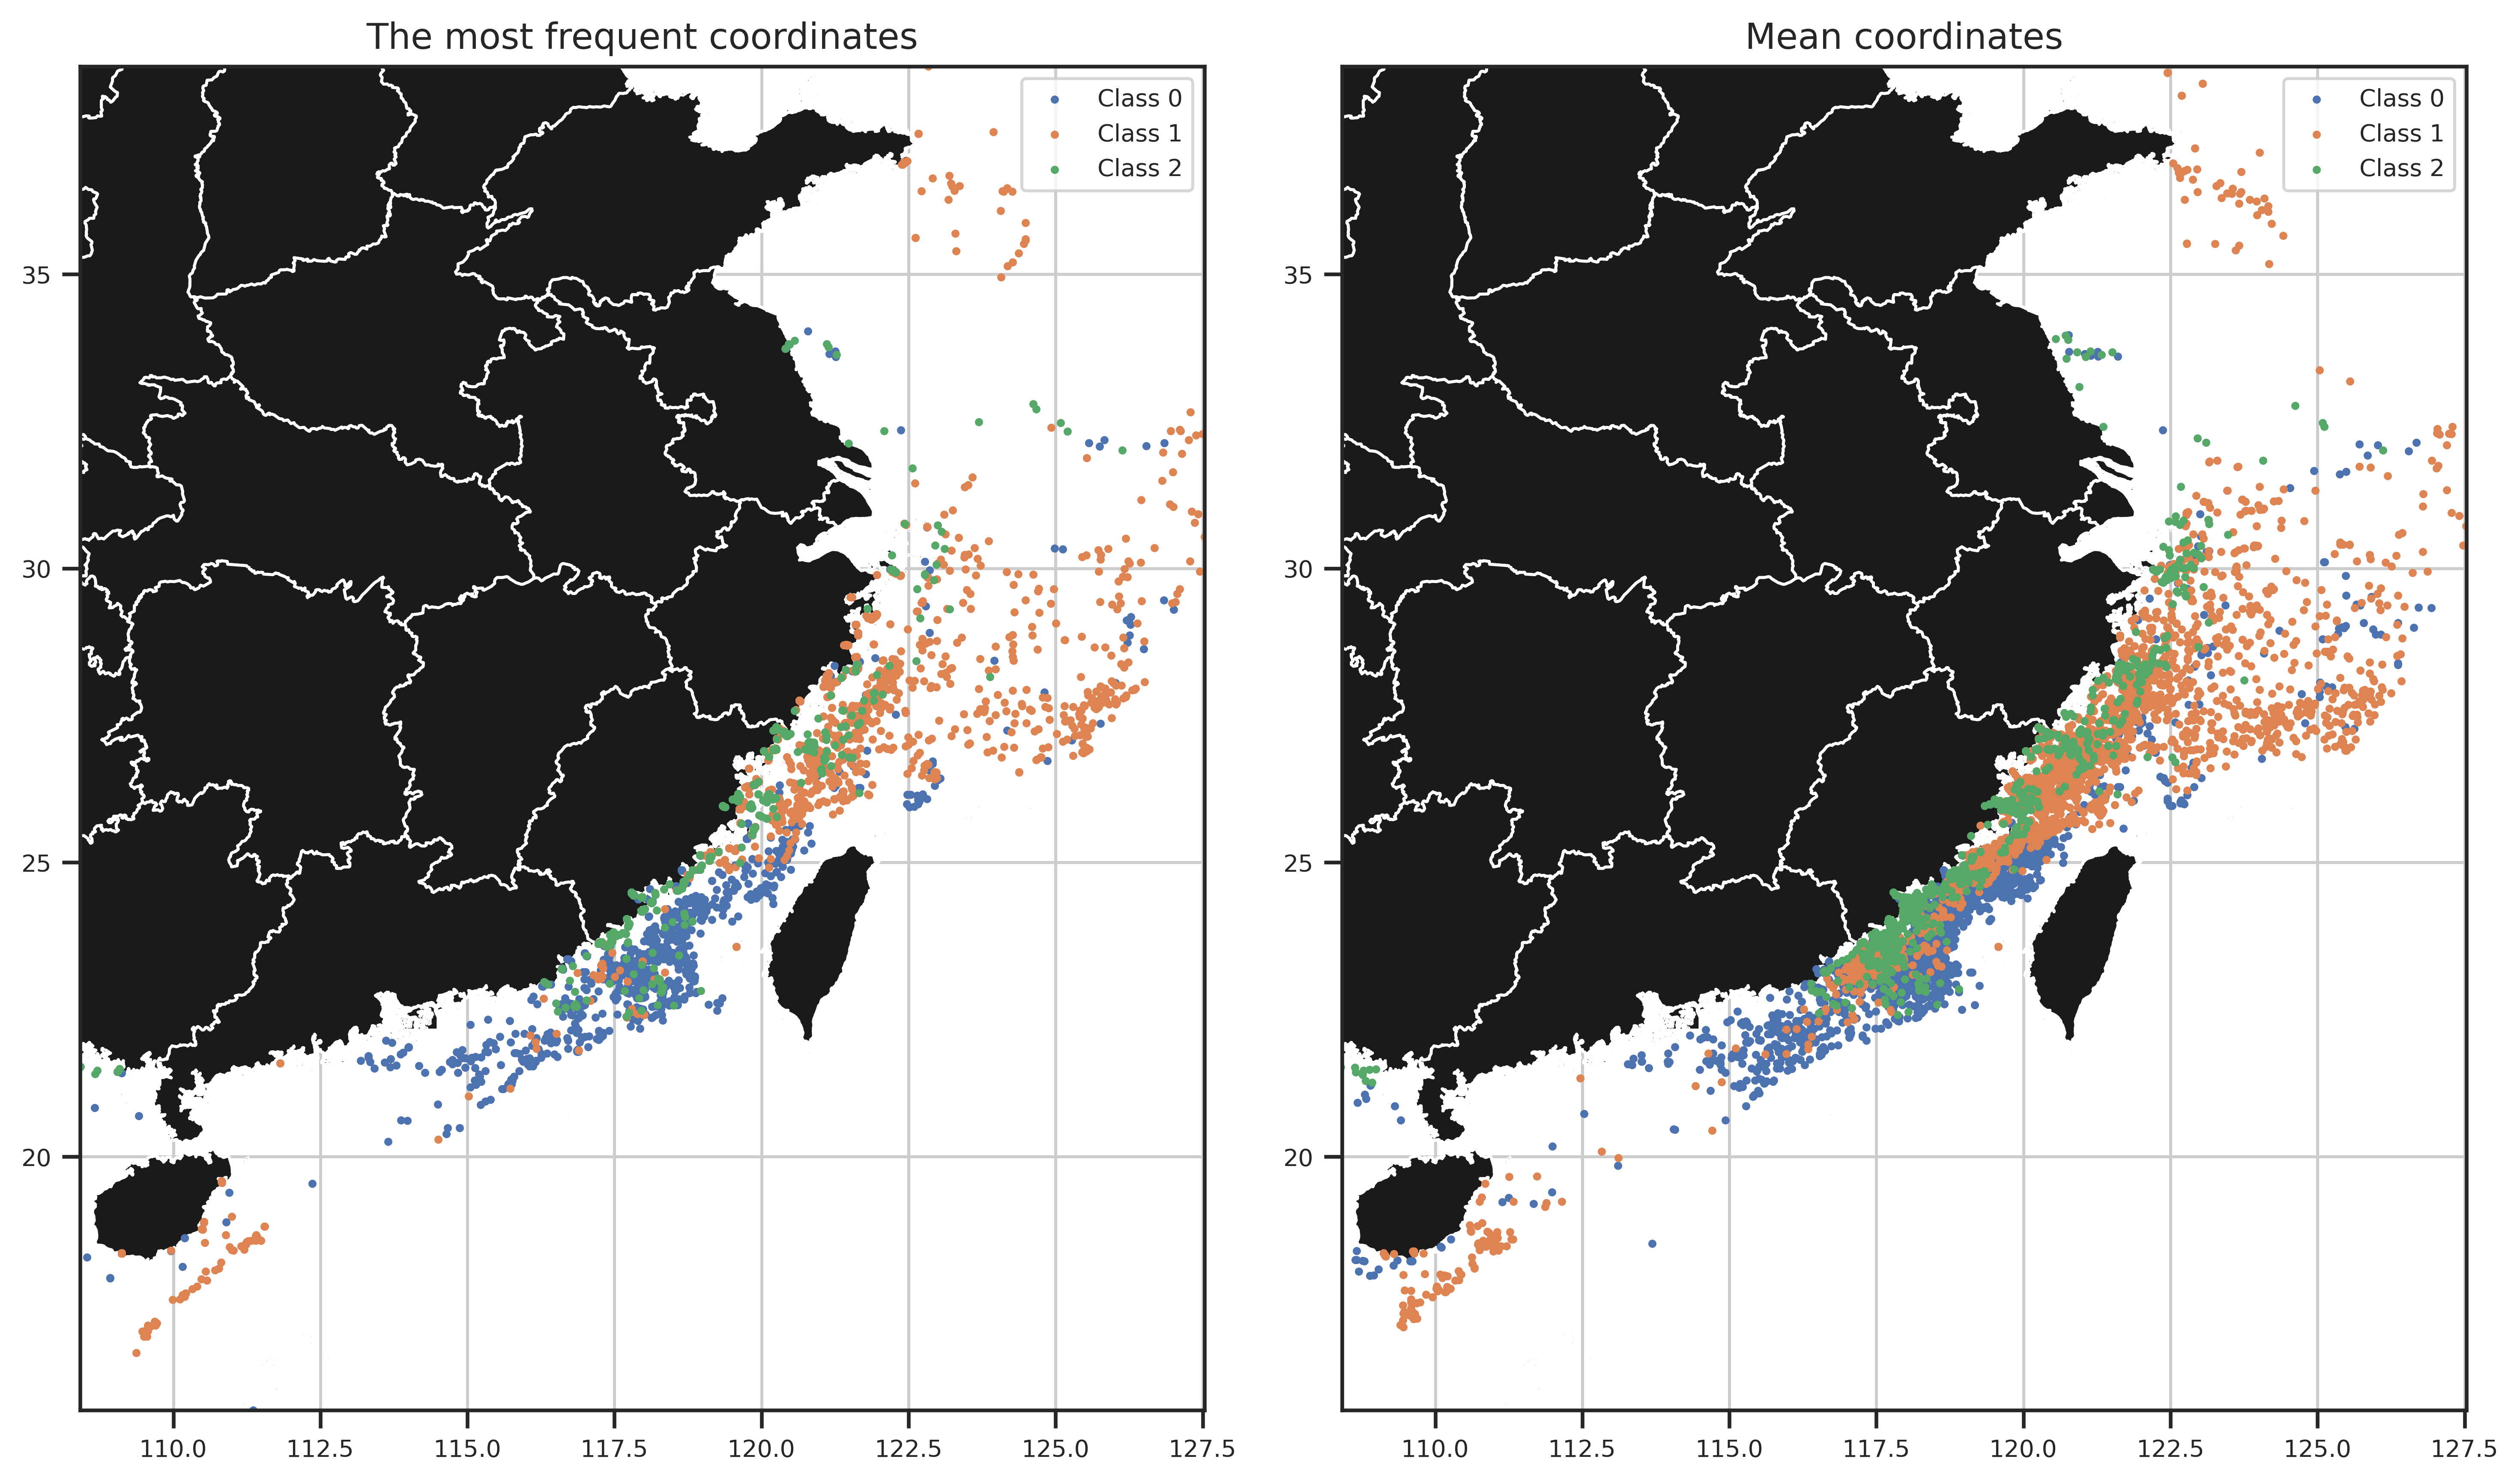
\includegraphics[width=0.75\linewidth]{..//plots//feature_mean_freq_coordinates.png}
		\caption{轨迹平均坐标与频繁坐标分布图}
		\label{sec_1_fig_7}
		\vspace{-0.2cm}
	\end{figure}
	由图(\ref{sec_1_fig_7})可以看出,不同类别的渔船明显存在不同的活动海域。即不同类别的渔船,在平面坐标系下,有着明显不同的活动海域,每条轨迹的最频繁样本图可以清晰看出该规律。这点可以直接作为分类模型的建模依据,后来也成为我们模型的强特之一。

%%%%%%%%%%%%%%%%%%%%%%%%%%%%%%%%%%%%%%%%%%%%
	\subsection{基础探索性分析总结}
	总的来说,通过基础数据的探索,我们得出了以下结论:
	\begin{enumerate}
		\item \textbf{轨迹数据中存在异常值。}不论是坐标序列还是轨迹速度序列,都存在异常值,因此需要对异常值进行修复。
		\item \textbf{轨迹的当中存在POI点,需要深入进行挖掘。}可视化的结果表示,轨迹中应当存在POI点以及POI点组成的ROI(Region of Interested)区域,需要通过特殊方法深入挖掘此类信息,从而细致的刻画渔船的运动特性。
		\item \textbf{不同类别轨迹速度存在明显差异性。}不同行为的轨迹,速度分布存在显著差异,对应于拖网围网与刺网的不同运动特性,可直接通过每条轨迹的分位数特征捕获这样的特征分布的差异性。
		\item \textbf{不同类别的轨迹方向的分布差异性不明显。}不同行为的轨迹,其方向的分布特性不明显,组织特征时,方向特征需要特殊处理。
		\item \textbf{坐标可直接作为区分不同行为轨迹的标准。}不同行为的渔船有着不同的活动海域,可能对应于不同的渔场,可以直接使用坐标对这样的信息进行捕获。
		\item \textbf{统计特征建模并不足够描述轨迹的特性。}单纯从统计的角度,并未捕获渔船运动序列的时序性,因此需要用特殊方法对渔船的运动特性进行建模。
	\end{enumerate}




%%%%%%%%%%%%%%%%%%%%%%%%%%%%%%%%%%%%%%%%%%%%
%%%%%%%%%%%%%%%%%%%%%%%%%%%%%%%%%%%%%%%%%%%%
	\section{算法阶段:渔船作业类型识别方法}\label{sec_2}
		本节我们详细介绍在初赛和复赛算法阶段的渔船作业类型识别部分采用的策略。

%%%%%%%%%%%%%%%%%%%%%%%%%%%%%%%%%%%%%%%%%%%%
		\subsection{数据清洗部分}
		首先,由于传感器采集误差的缘故会导致真实轨迹数据中存在异常轨迹点,误差不仅反映在轨迹坐标记录中,也反映在传感器读数的记录中。因此需要事先采取合适的方法来进行数据清洗,其中数据清洗的目标如下:
		\begin{enumerate}
			\item 能够识别全局异常与局部异常的轨迹坐标的读数,例如离群的轨迹点,局部的由于传感器跳变导致的异常坐标读数。
			\item 能够识别异常的渔船速度记录,例如渔船某个时刻速度达到100节以上。
			\item 需要根据情况修复异常的坐标与异常的速度值。
		\end{enumerate}

		\begin{figure}[H]
			\centering
			\begin{tabular}{ccc}
				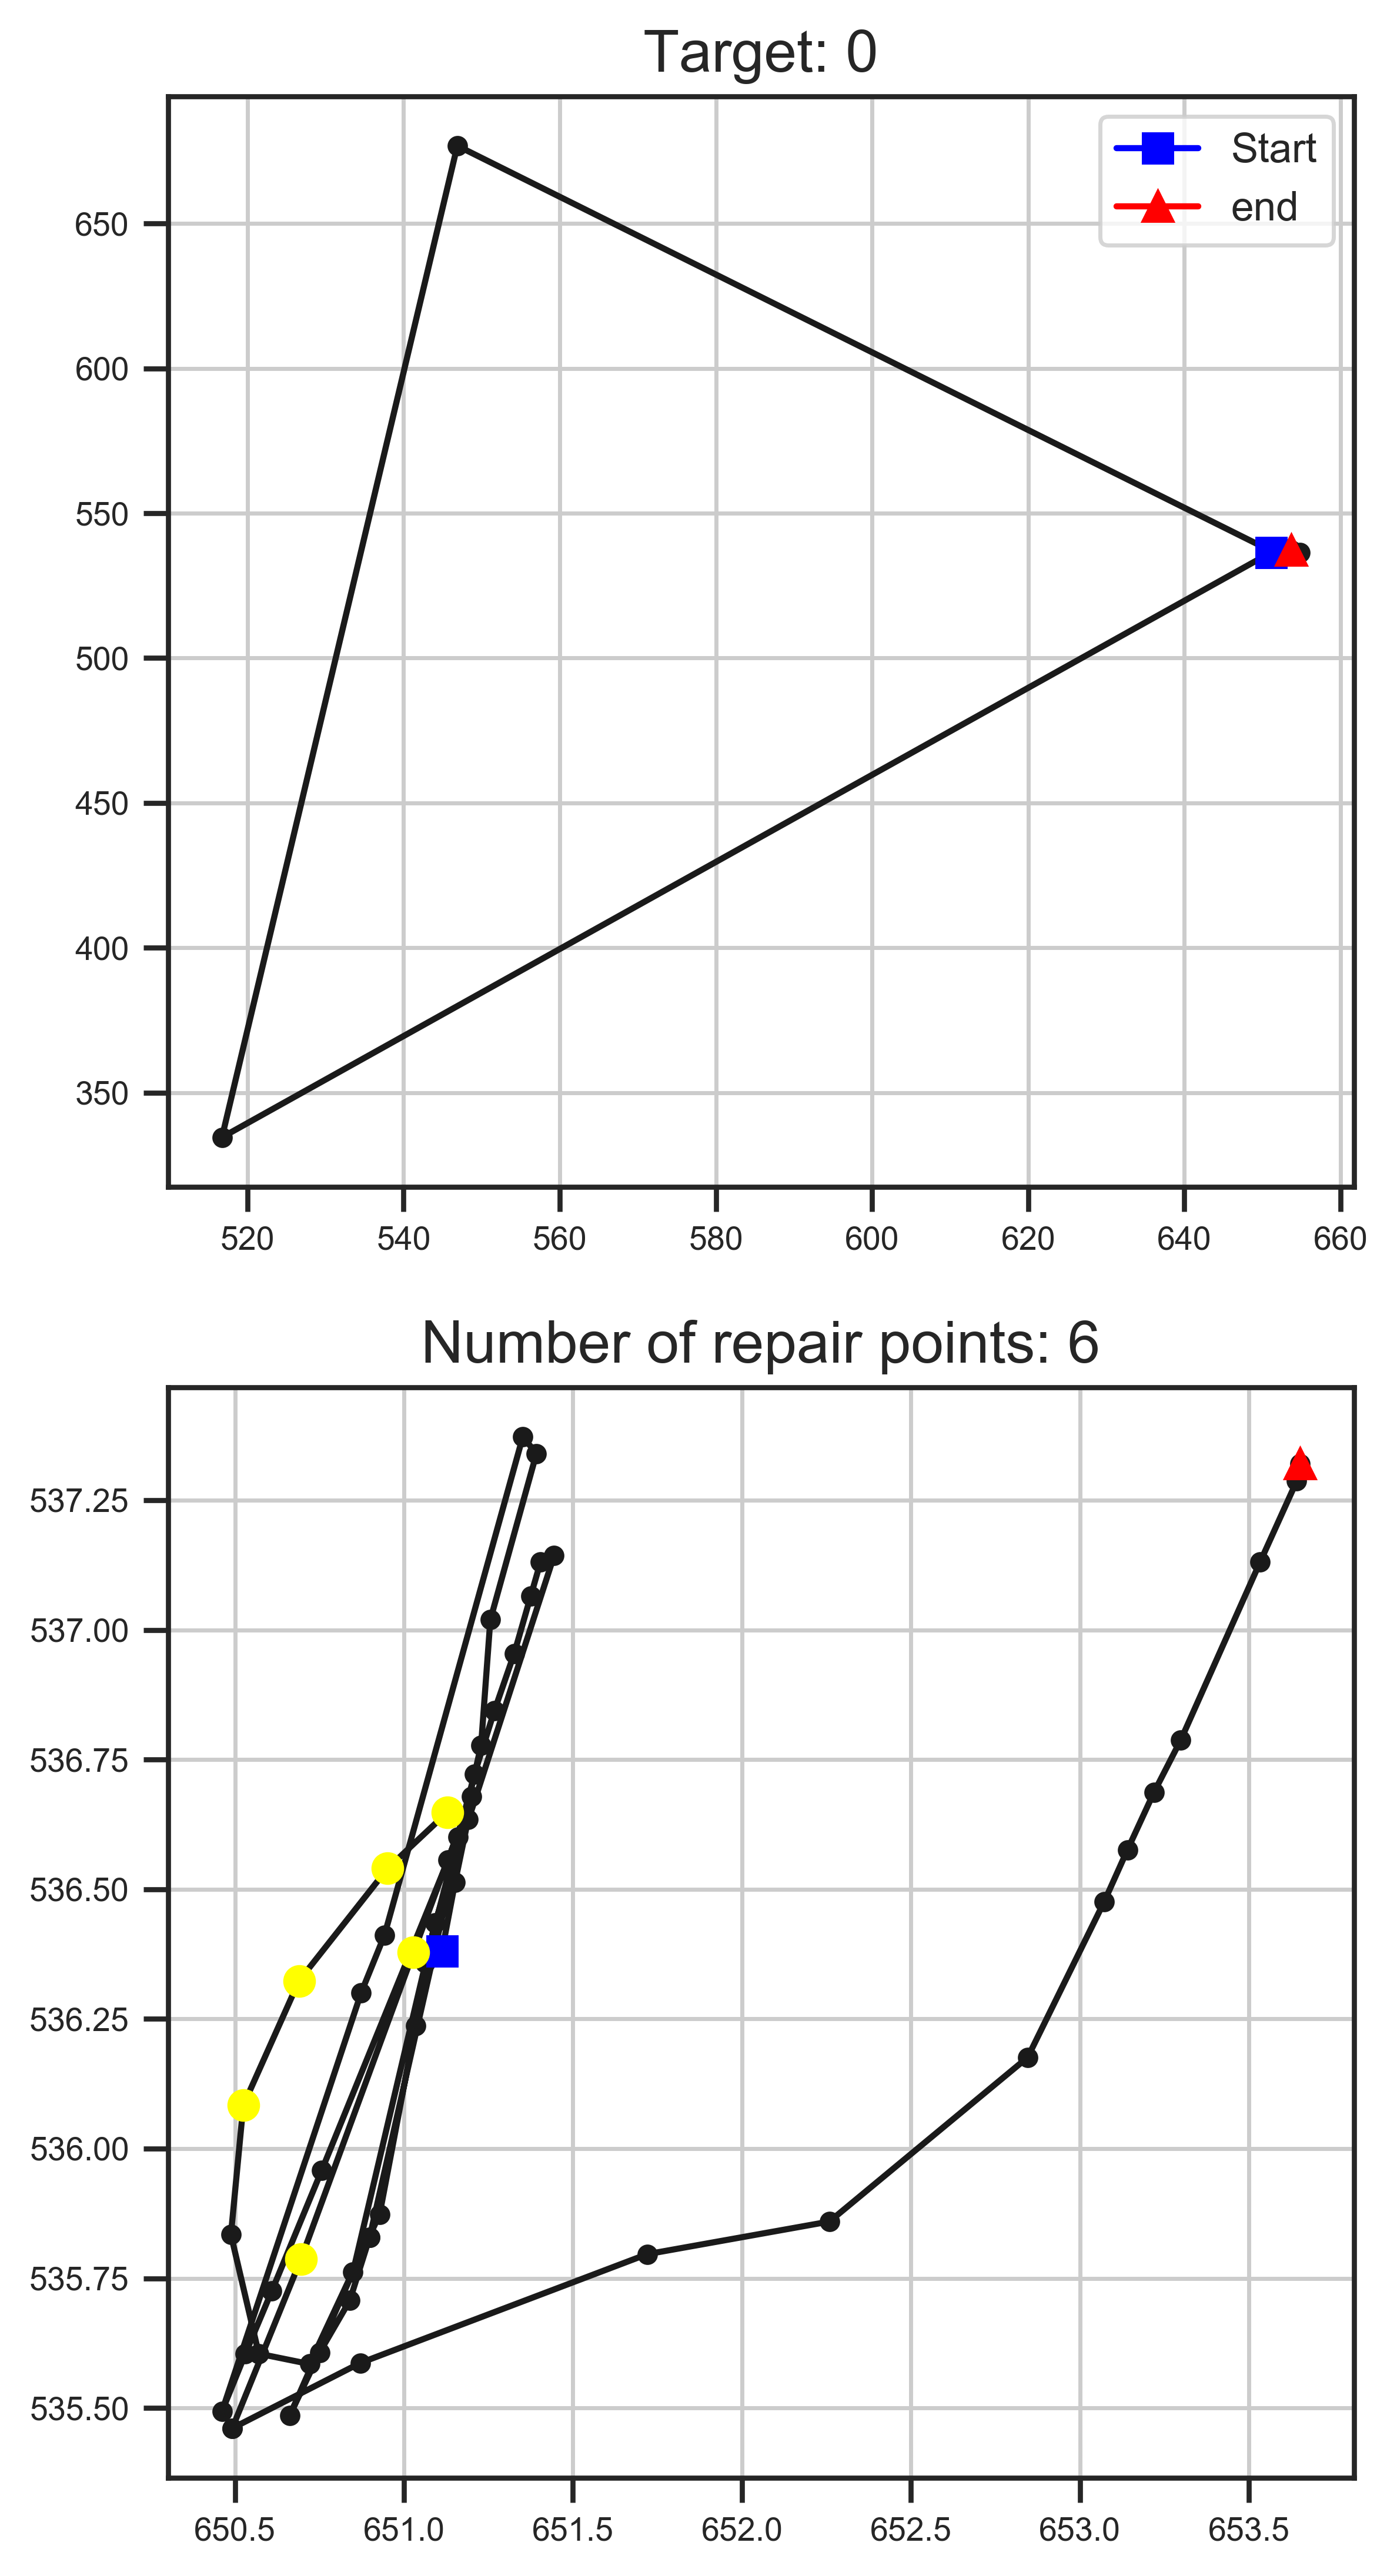
\includegraphics[width=0.27\linewidth]{..//plots//traj_filtering_396.png} & 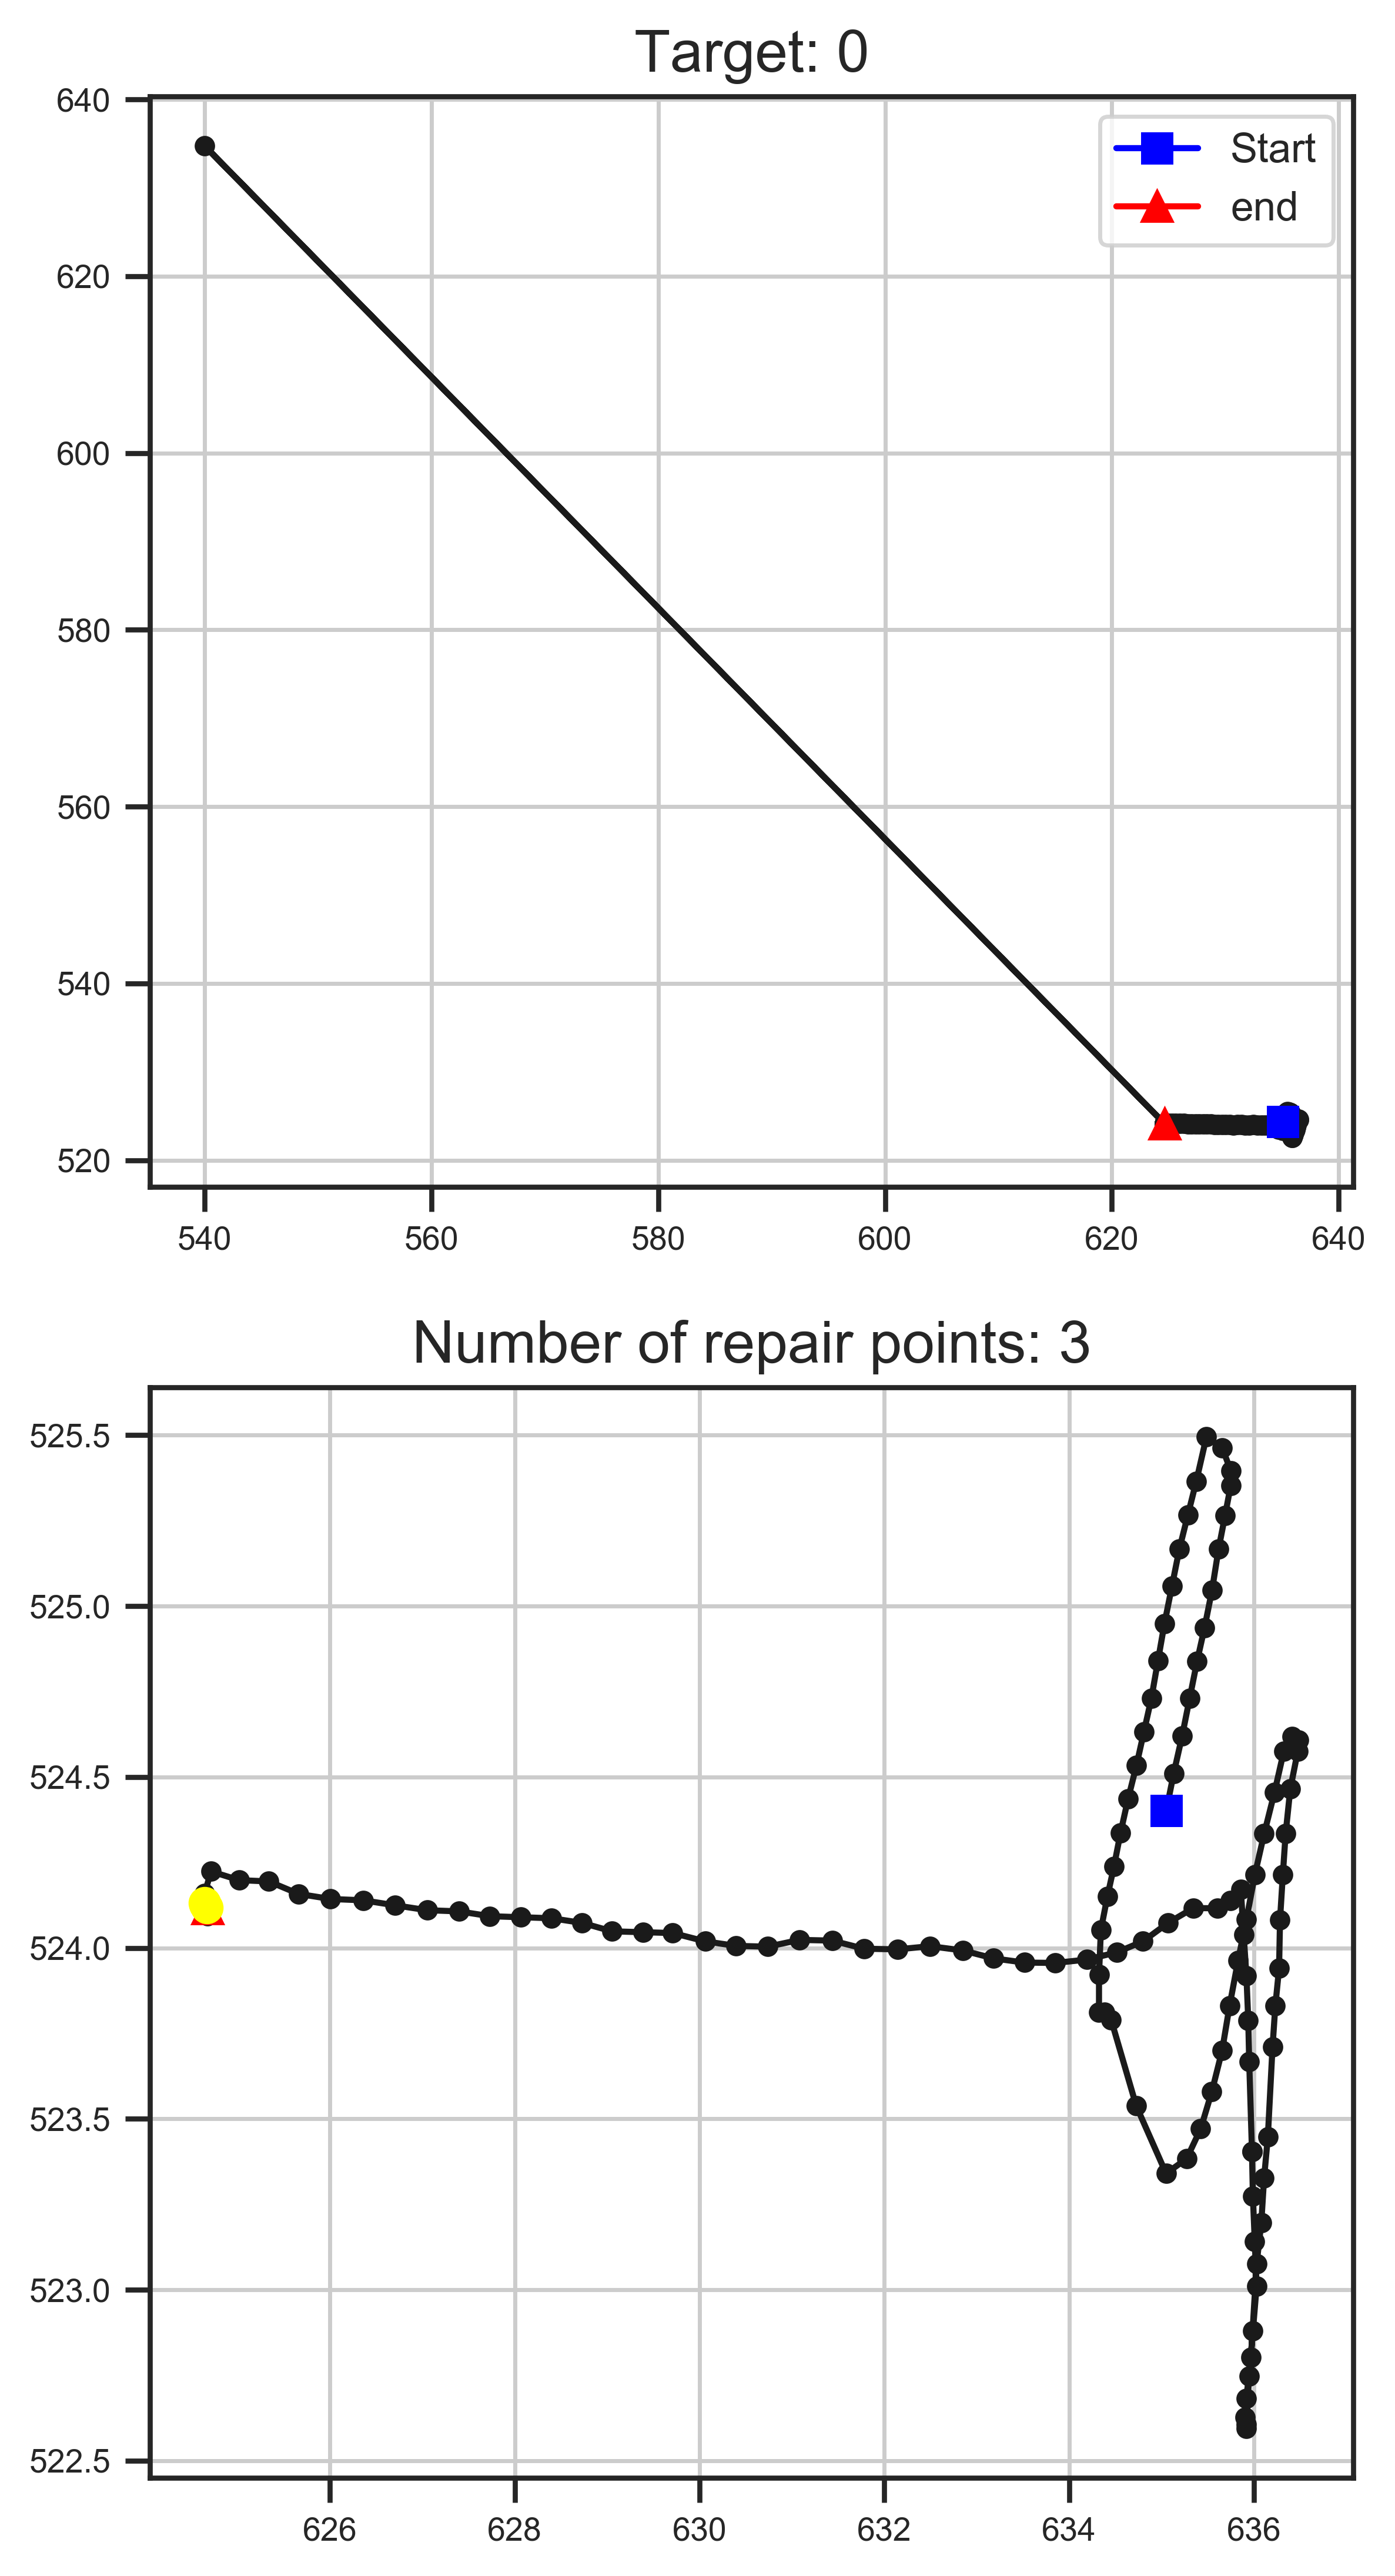
\includegraphics[width=0.27\linewidth]{..//plots//traj_filtering_691.png} &
				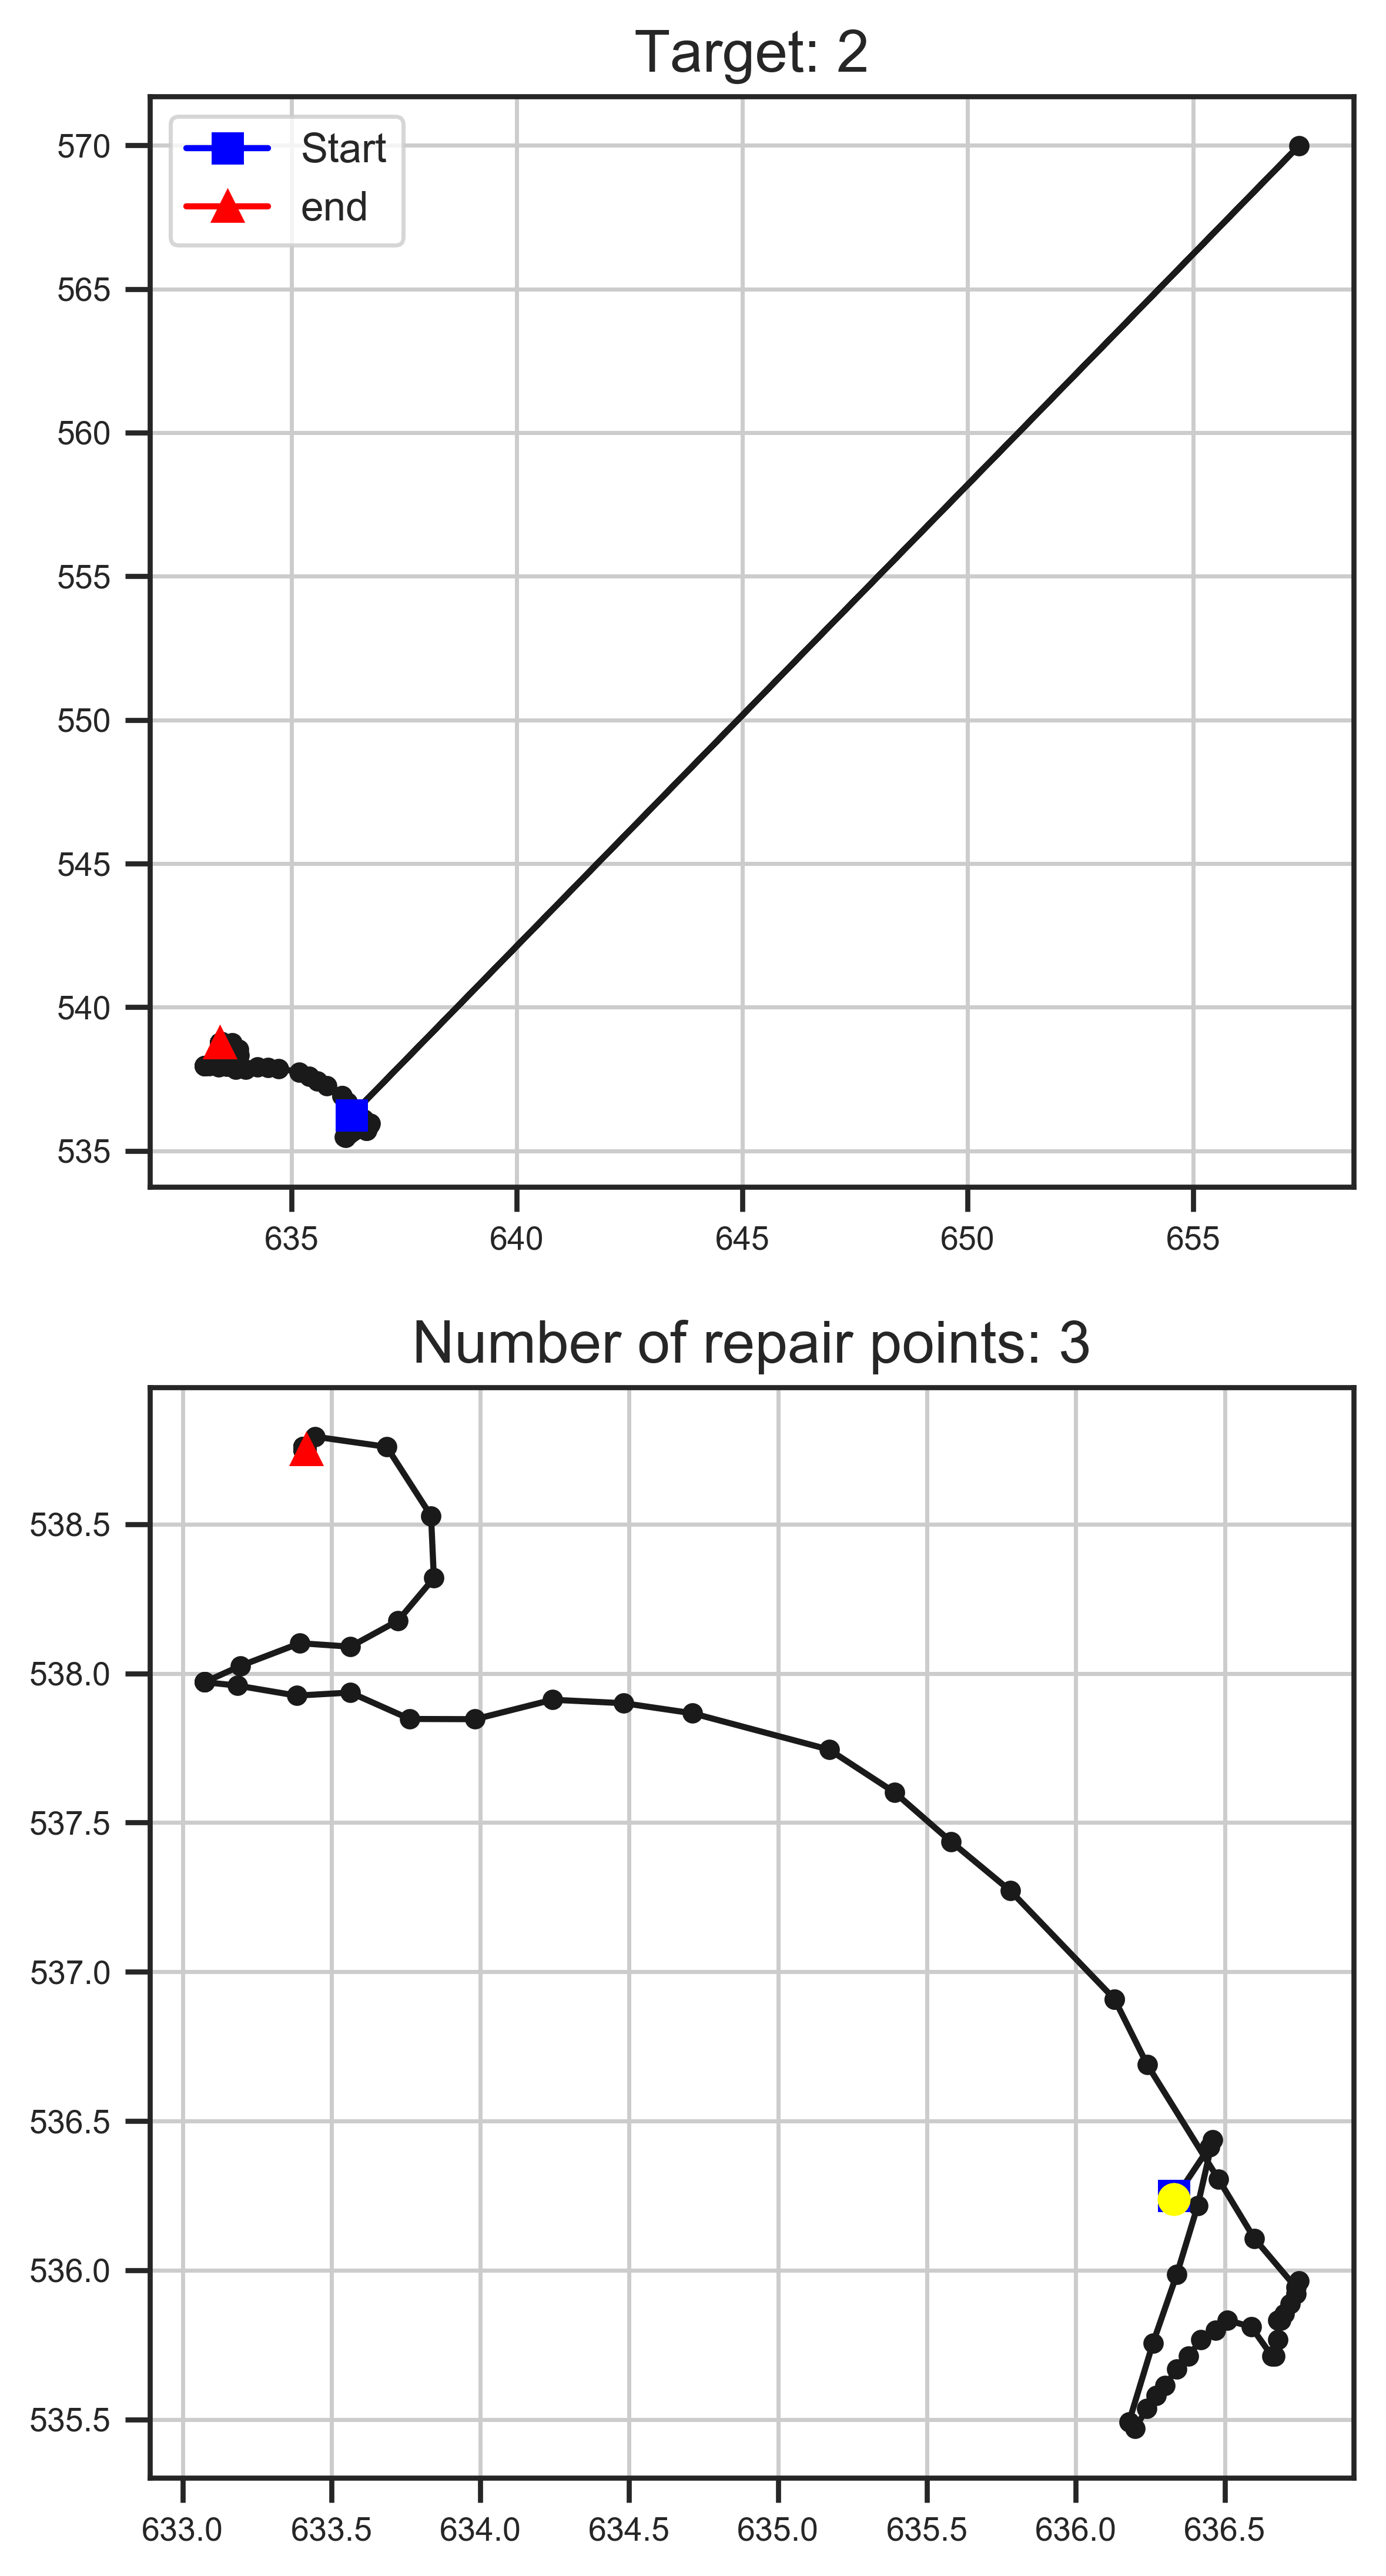
\includegraphics[width=0.27\linewidth]{..//plots//traj_filtering_1093.png} \\
				(a) & (b) & (c)
			\end{tabular}
			\caption{修复后的轨迹}
			\label{sec_2_fig_0}
			\vspace{-0.2cm}
		\end{figure}
		在预处理阶段,我们首先将每一条轨迹的坐标由WGS-84转换到了EPSG-3395坐标系下,方便后续坐标距离的计算;其次我们计算了每条轨迹坐标点之间的差分haversine距离,并以此计算了局部差分速度,并依据局部差分速度,依据事先给定阈值识别了异常坐标;最后,基于预设的最大速度阈值,对超过阈值的速度和坐标进行了多项式插值,补全缺失信息。图(\ref{sec_2_fig_0})是离群轨迹点插值结果。

%%%%%%%%%%%%%%%%%%%%%%%%%%%%%%%%%%%%%%%%%%%%
		\subsection{POI信息挖掘}
		为了更为细致的刻画轨迹的运动部分的模式,也为了后续渔船的用户画像的构建,我们对POI点信息进行了挖掘。比赛中采用了比较简单的方法对POI信息进行挖掘,首先我们将每条轨迹投射到了一个网格坐标系下。图(\ref{sec_2_grid_compression})是投射方法。
		\begin{figure}[H]
			\centering
			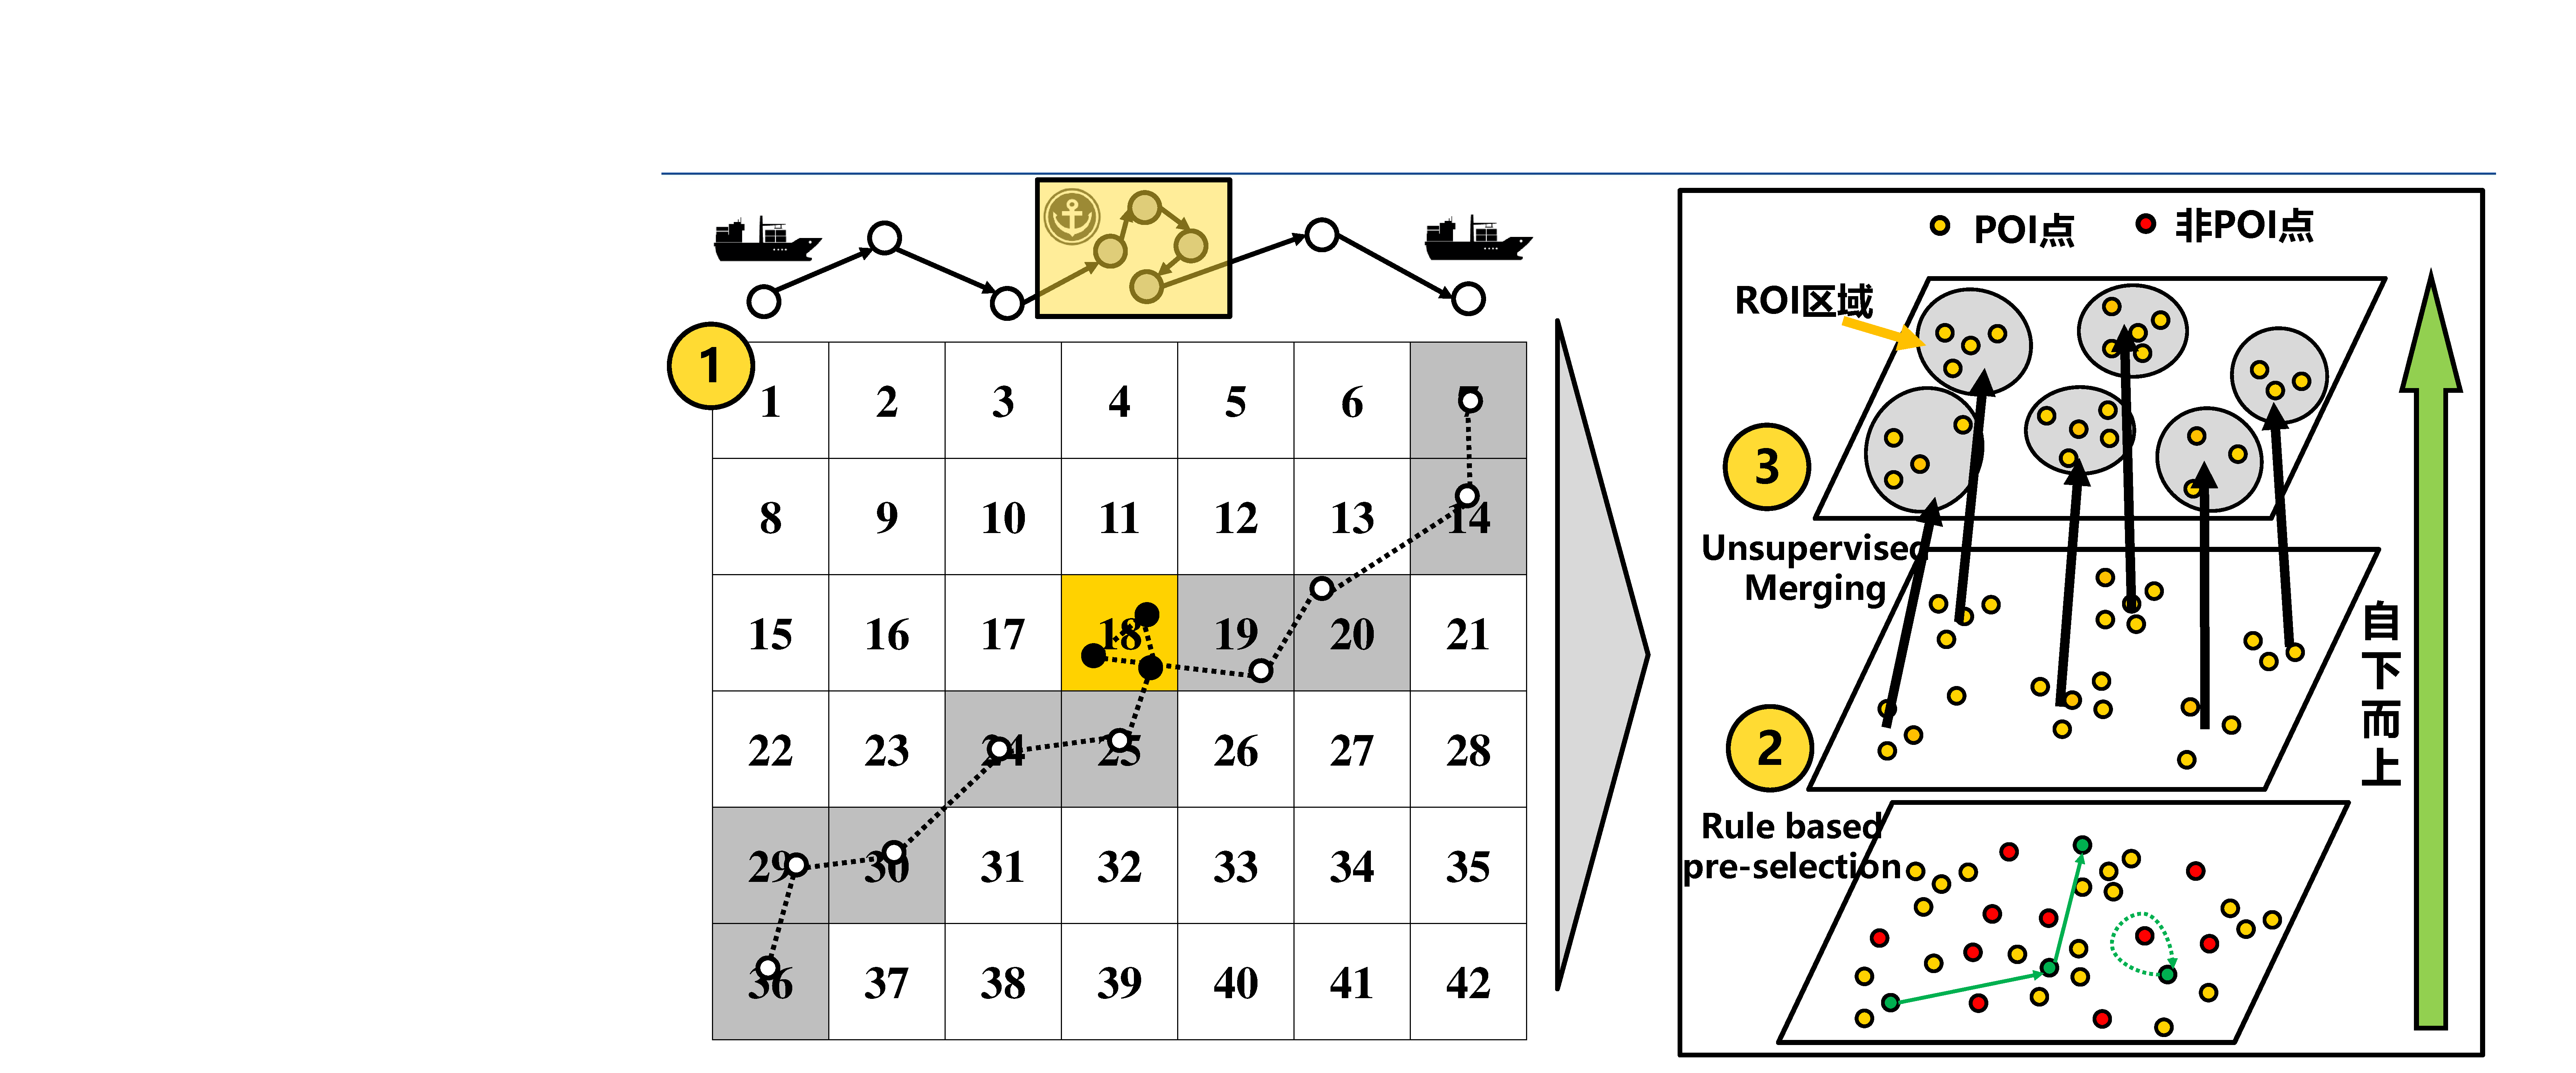
\includegraphics[width=0.55\linewidth]{..//plots//poi_mining_method.pdf}
			\caption{轨迹被投射到网格上,轨迹坐标序列成为了坐标编号序列}
			\label{sec_2_grid_compression}
			\vspace{-0.2cm}
		\end{figure}
		随后我们基于被id不同的渔船访问次数(unique visit count),不同id的渔船在该网格停留的平均时长(mean stay time)和网格总的被访问的次数(total visit count)三个指标,筛选出了一系列的POI网格。这一轮筛选后可以得到了潜在的POI网格的编号与坐标,最后我们使用DBSCAN对这些网格坐标进行了一次聚类,合并了具有相近地理位置的网格。
		\begin{figure}[H]
			\centering
			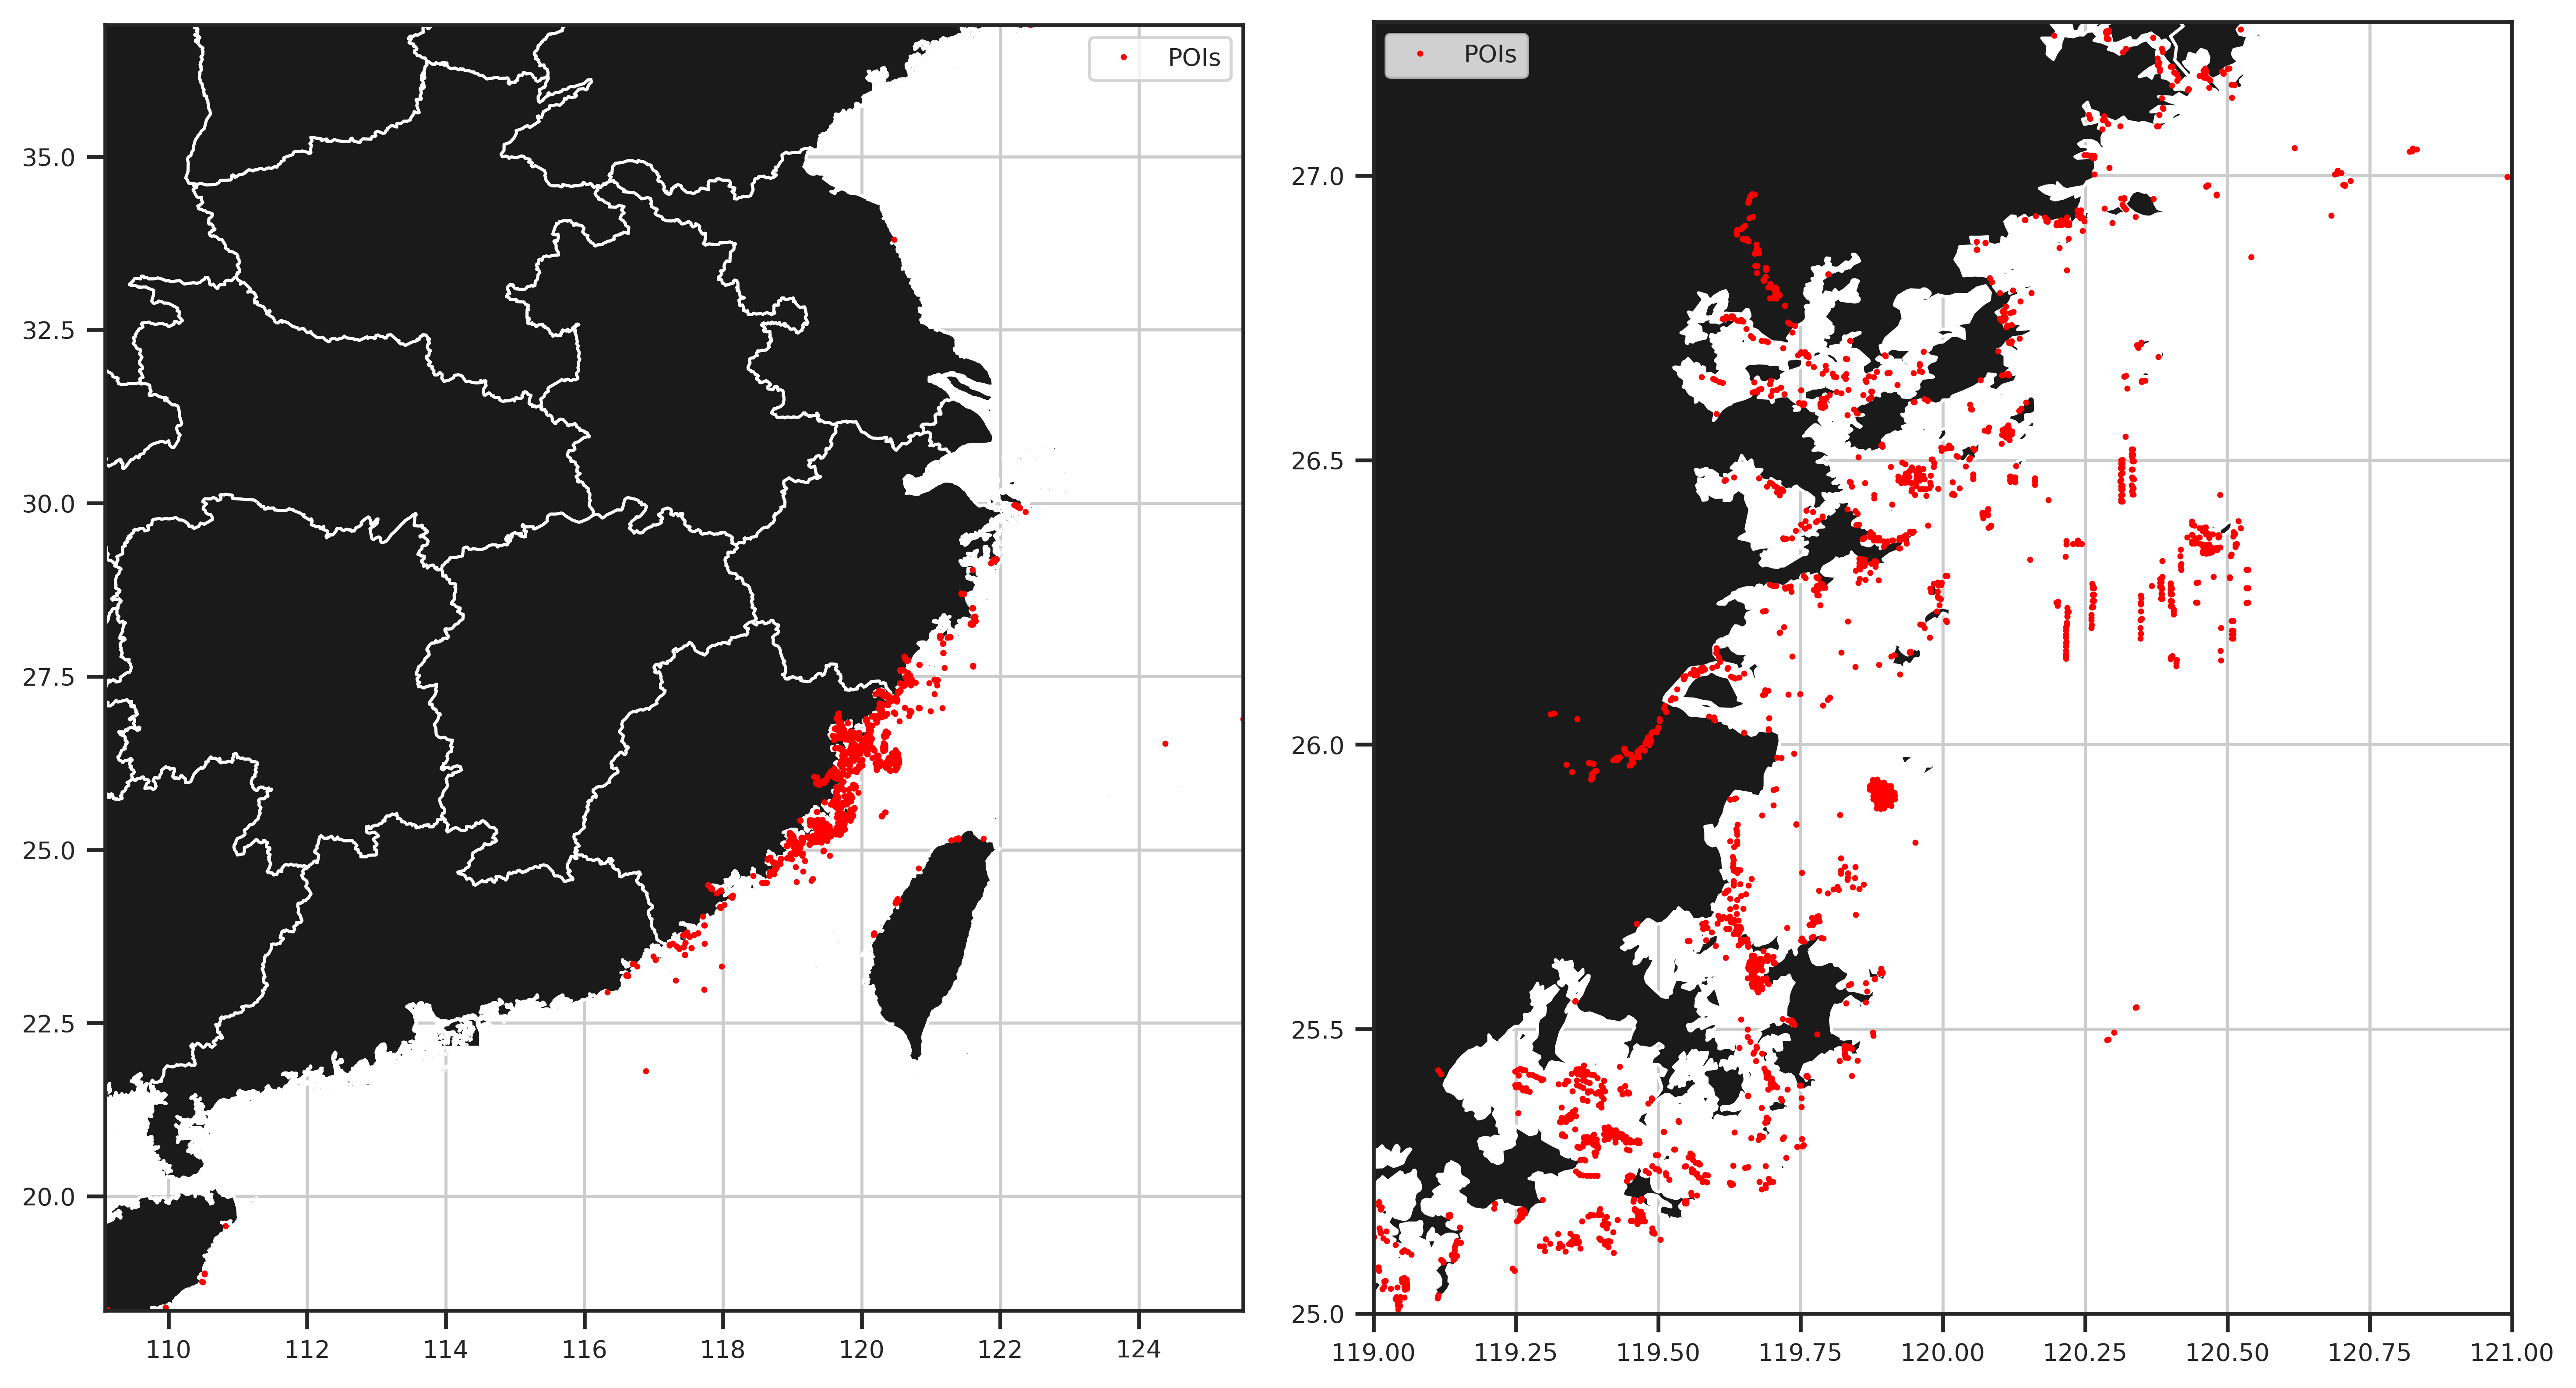
\includegraphics[width=0.7\linewidth]{..//plots//feature_pois.png}
			\caption{POI点图,可见有一些访问热点位于海上,对应可能的渔区}
			\label{sec_2_fig_1}
			\vspace{-0.2cm}
		\end{figure}
		图(\ref{sec_2_fig_1})为我们提出的方法抽取的POI点。比赛中我们也试图使用聚类方法获取POI信息,总的来说效果不如基于规则的方法稳定。在经过这一步处理之后,每一条轨迹的每一个轨迹点都拥有了其所属的POI标签。

%%%%%%%%%%%%%%%%%%%%%%%%%%%%%%%%%%%%%%%%%%%%
		\subsection{基于word2vec的轨迹时序信息挖掘方法}
		上一节中我们将每条轨迹转换为了网格坐标的序列。因此自然可以使用word2vec来捕获轨迹的时序特性。在比赛当中我们进行了坐标序列和传感器采集的序列都进行了embedding。对于第一种embedding,我们将其称为traj2vec,也就是轨迹向量化。在该组embedding过程中,我们直接使用CBOW获取每个词的词向量;随后对于轨迹的向量表示而言,是其所包含的词(网格)向量的平均。
		\begin{figure}[H]
			\centering
			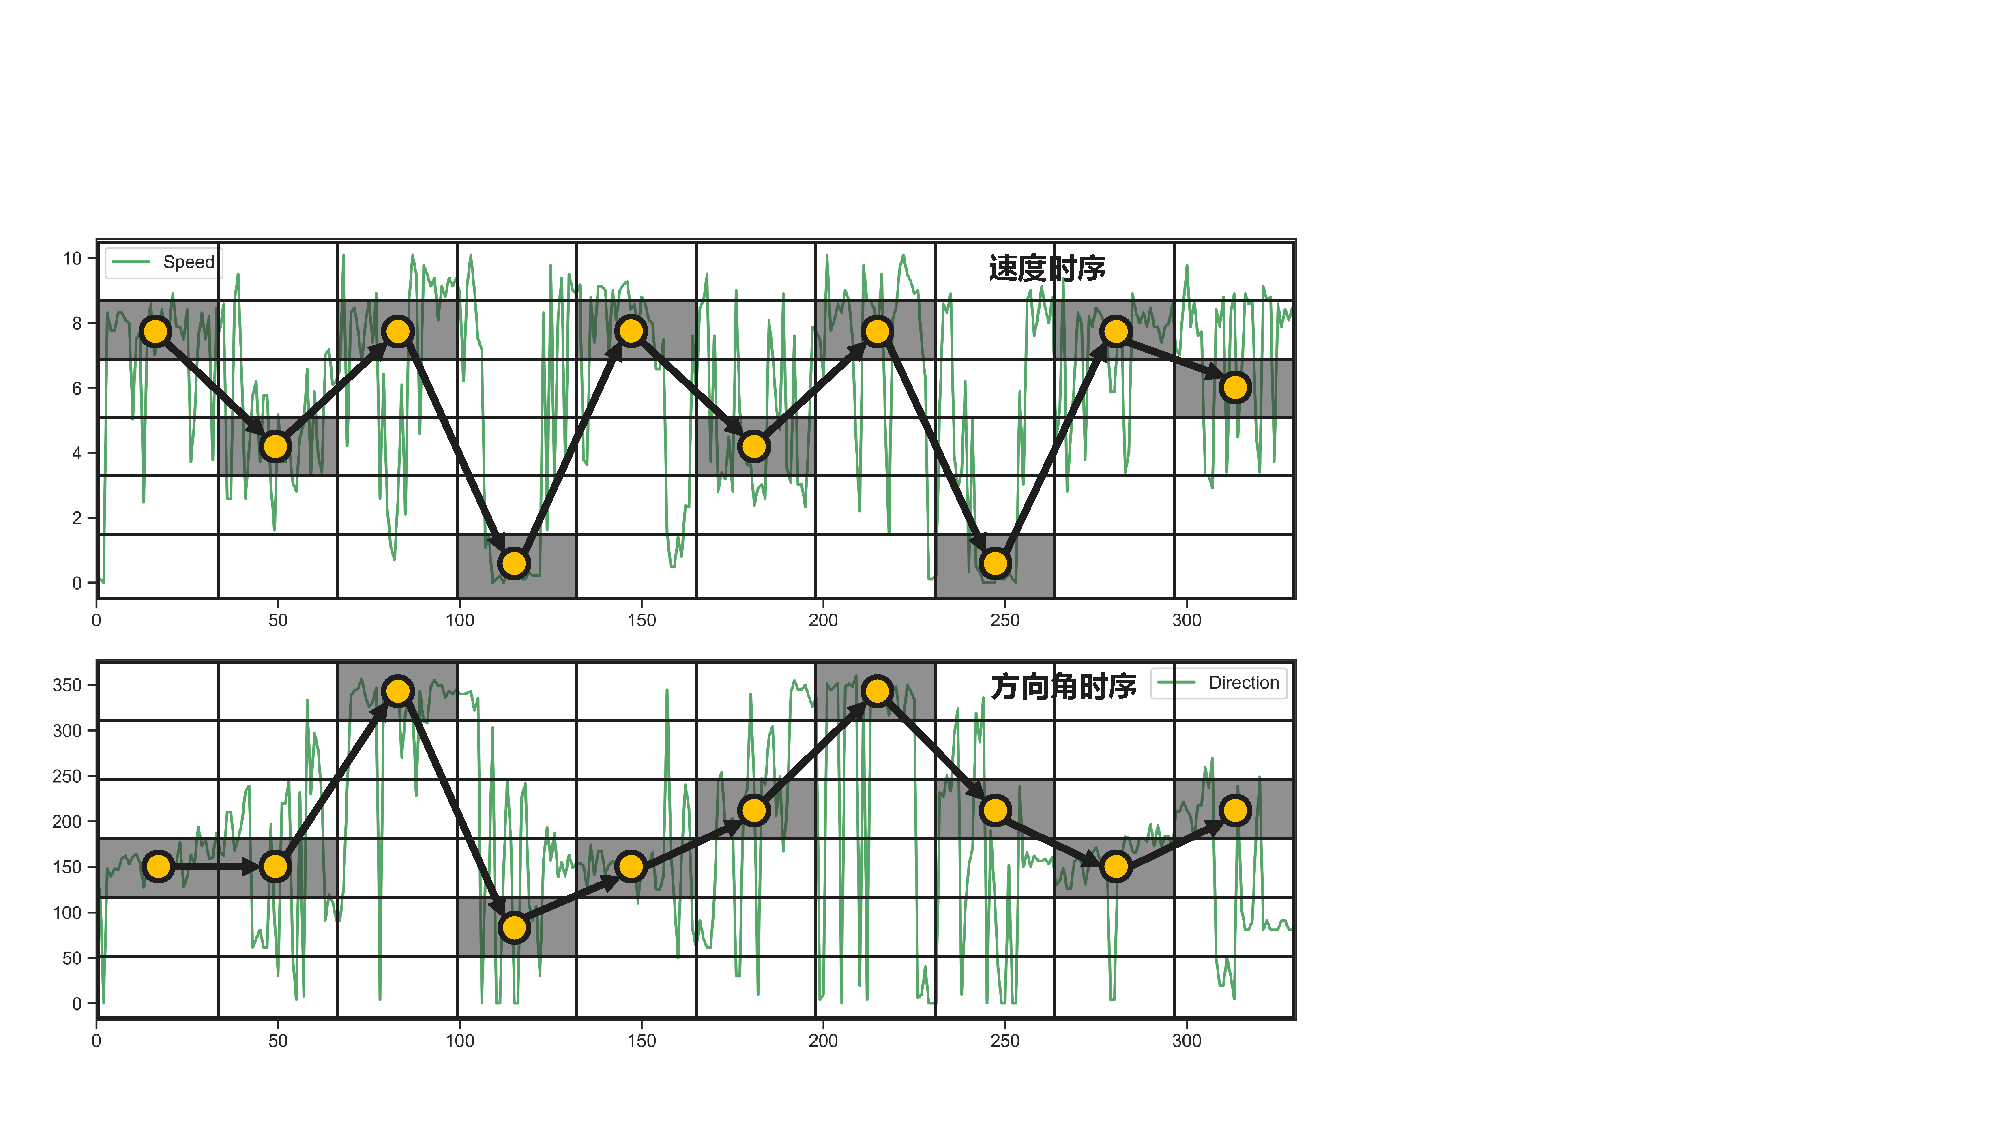
\includegraphics[width=0.7\linewidth]{..//plots//sequence_encoding.pdf}
			\caption{传感器时序的embedding}
			\label{sec_2_sequence_encoding}
			\vspace{-0.2cm}
		\end{figure}
		第二组embedding如图(\ref{sec_2_sequence_encoding})所示,我们将轨迹的速度序列和方向序列也进行了embedding的操作。通过这样的方法捕获了样本的速度与方向时序的性质。

%%%%%%%%%%%%%%%%%%%%%%%%%%%%%%%%%%%%%%%%%%%%
		\subsection{轨迹统计信息挖掘方法}
		上一节中,不论是traj2vec还是传感器序列信息的embedding都只捕获了时序性,我们也设计了一系列的统计特征抽取每条轨迹的dense features。具体来说,对于每条轨迹而言:
		\begin{enumerate}
			\item 抽取轨迹经度与纬度以及他们的一些经纬度交叉(不在POI点的轨迹点)的分位数特征。
			\item 抽取轨迹经纬度的运动部分的统计特征(不在POI点的轨迹点),例如均值,方差,最大值减最小值等。这些特征用于刻画渔船细节的一系列运动特性,用于捕获拖网围网与刺网捕捞的运动特性的区别。
			\item 抽取了轨迹的最频繁点。非常强的强特,猜测可能与渔船活动区域对应的渔场有关。
			\item 不在POI点处的轨迹点的速度的分位数特征。
			\item 渔船的活动范围等特殊的专家特征。
		\end{enumerate}
		在获取了dense features之后,我们将其与embedding特征进行结合,用来训练分类器。

%%%%%%%%%%%%%%%%%%%%%%%%%%%%%%%%%%%%%%%%%%%%
		\subsection{半监督学习强化与分类器训练}
		我们采用了半监督学习里较为简单的一个策略来强化模型的稳定性。图(\ref{sec_2_fake_labels})为我们的策略基本说明。
		\begin{figure}[H]
			\centering
			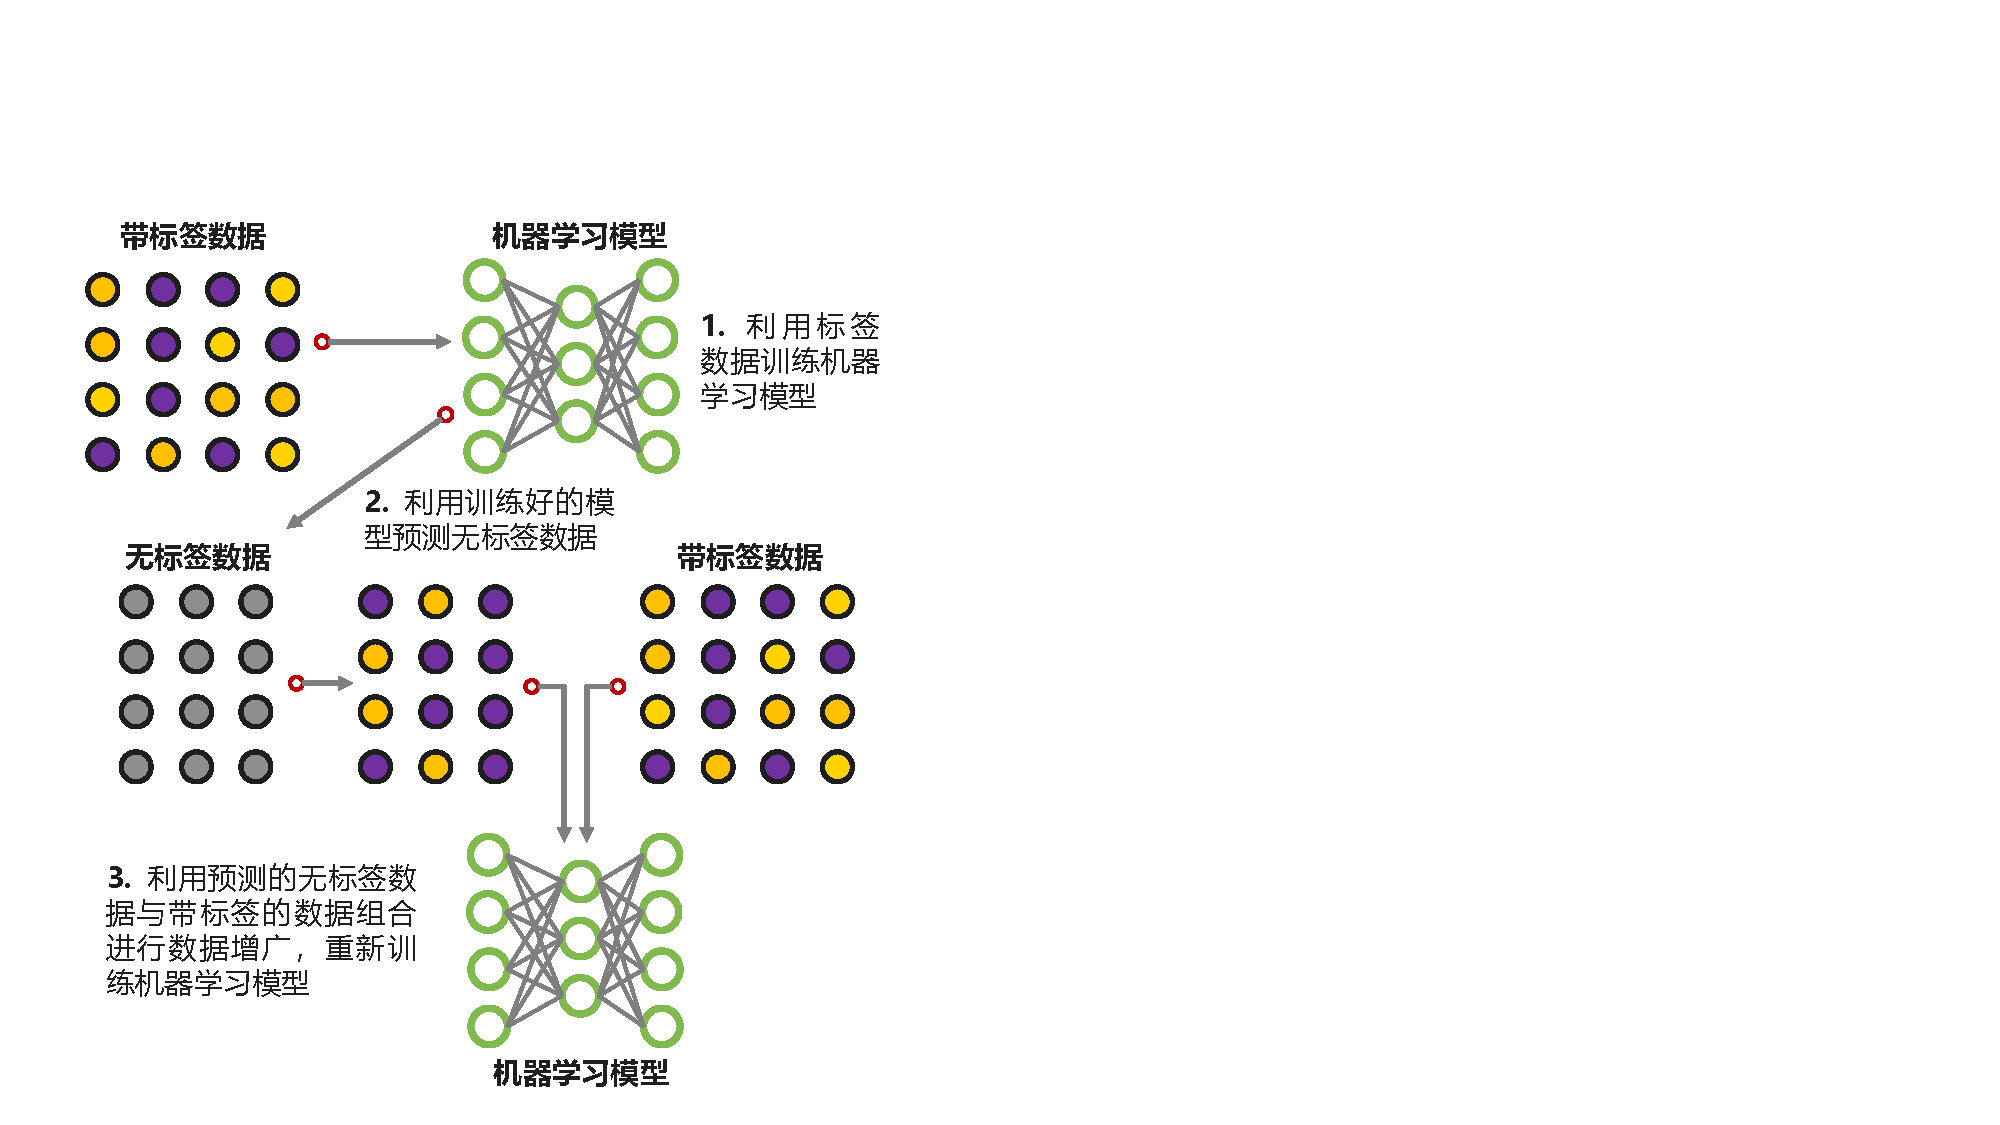
\includegraphics[width=0.55\linewidth]{..//plots//fake_labels.pdf}
			\caption{传感器时序的embedding}
			\label{sec_2_fake_labels}
			\vspace{-0.2cm}
		\end{figure}
		在实际比赛中,半监督学习扮演了一个较为关键的决赛,在复赛算法的B阶段,通过半监督学习,线上F1分数由0.889跃升到了0.8995。


%%%%%%%%%%%%%%%%%%%%%%%%%%%%%%%%%%%%%%%%%%%%
		\section{总结}\label{sec_3}
		本节中,我们简述了应用于渔船作业类型分类的数据清洗,特征组织的相关工作。特征工程从时序性与统计特征两个方面对不同类型的轨迹的运动特性进行了建模。整个特征工程采用了多进程并行,在我们的设备上时间控制在5分钟以内;对于整个模型训练过程而言,embedding部分花费大概20分钟左右,分类器的训练花费的时间大概在1到2分钟左右。通过细致的特征工程,我们在初赛阶段单模便到达过0.9111的分数,排名排行榜第一位。这样说明了我们特征工程的充分性。

	\bibliographystyle{unsrt}
	\bibliography{Final_ref}

\end{document}